\documentclass[a4paper]{article}

\def\npart {III}
\def\nterm {Lent}
\def\nyear {2017}
\def\nlecturer {A. J. Scholl}
\def\ncourse {Modular Forms and L-functions}
\def\nlectures {TTW.11}

% Imports
\ifx \nextra \undefined
  \usepackage[pdftex,
    hidelinks,
    pdfauthor={Dexter Chua},
    pdfsubject={Cambridge Maths Notes: Part \npart\ - \ncourse},
    pdftitle={Part \npart\ - \ncourse},
  pdfkeywords={Cambridge Mathematics Maths Math \npart\ \nterm\ \nyear\ \ncourse}]{hyperref}
  \title{Part \npart\ - \ncourse}
\else
  \usepackage[pdftex,
    hidelinks,
    pdfauthor={Dexter Chua},
    pdfsubject={Cambridge Maths Notes: Part \npart\ - \ncourse\ (\nextra)},
    pdftitle={Part \npart\ - \ncourse\ (\nextra)},
  pdfkeywords={Cambridge Mathematics Maths Math \npart\ \nterm\ \nyear\ \ncourse\ \nextra}]{hyperref}

  \title{Part \npart\ - \ncourse \\ {\Large \nextra}}
\fi

\author{Lectured by \nlecturer \\\small Notes taken by Dexter Chua}
\date{\nterm\ \nyear}

\usepackage{alltt}
\usepackage{amsfonts}
\usepackage{amsmath}
\usepackage{amssymb}
\usepackage{amsthm}
\usepackage{booktabs}
\usepackage{caption}
\usepackage{enumitem}
\usepackage{fancyhdr}
\usepackage{graphicx}
\usepackage{mathtools}
\usepackage{microtype}
\usepackage{multirow}
\usepackage{pdflscape}
\usepackage{pgfplots}
\usepackage{siunitx}
\usepackage{tabularx}
\usepackage{tikz}
\usepackage{tkz-euclide}
\usepackage[normalem]{ulem}
\usepackage[all]{xy}

\pgfplotsset{compat=1.12}

\pagestyle{fancyplain}
\lhead{\emph{\nouppercase{\leftmark}}}
\ifx \nextra \undefined
  \rhead{
    \ifnum\thepage=1
    \else
      \npart\ \ncourse
    \fi}
\else
  \rhead{
    \ifnum\thepage=1
    \else
      \npart\ \ncourse\ (\nextra)
    \fi}
\fi
\usetikzlibrary{arrows}
\usetikzlibrary{decorations.markings}
\usetikzlibrary{decorations.pathmorphing}
\usetikzlibrary{positioning}
\usetikzlibrary{fadings}
\usetikzlibrary{intersections}
\usetikzlibrary{cd}

\newcommand*{\Cdot}{\raisebox{-0.25ex}{\scalebox{1.5}{$\cdot$}}}
\newcommand {\pd}[2][ ]{
  \ifx #1 { }
    \frac{\partial}{\partial #2}
  \else
    \frac{\partial^{#1}}{\partial #2^{#1}}
  \fi
}

% Theorems
\theoremstyle{definition}
\newtheorem*{aim}{Aim}
\newtheorem*{axiom}{Axiom}
\newtheorem*{claim}{Claim}
\newtheorem*{cor}{Corollary}
\newtheorem*{defi}{Definition}
\newtheorem*{eg}{Example}
\newtheorem*{fact}{Fact}
\newtheorem*{law}{Law}
\newtheorem*{lemma}{Lemma}
\newtheorem*{notation}{Notation}
\newtheorem*{prop}{Proposition}
\newtheorem*{thm}{Theorem}

\renewcommand{\labelitemi}{--}
\renewcommand{\labelitemii}{$\circ$}
\renewcommand{\labelenumi}{(\roman{*})}

\let\stdsection\section
\renewcommand\section{\newpage\stdsection}

% Strike through
\def\st{\bgroup \ULdepth=-.55ex \ULset}

% Maths symbols
\newcommand{\bra}{\langle}
\newcommand{\ket}{\rangle}

\newcommand{\N}{\mathbb{N}}
\newcommand{\Z}{\mathbb{Z}}
\newcommand{\Q}{\mathbb{Q}}
\renewcommand{\H}{\mathbb{H}}
\newcommand{\R}{\mathbb{R}}
\newcommand{\C}{\mathbb{C}}
\newcommand{\Prob}{\mathbb{P}}
\renewcommand{\P}{\mathbb{P}}
\newcommand{\E}{\mathbb{E}}
\newcommand{\F}{\mathbb{F}}
\newcommand{\cU}{\mathcal{U}}
\newcommand{\RP}{\mathbb{RP}}
\newcommand{\CP}{\mathbb{CP}}

\newcommand{\ph}{\,\cdot\,}

\DeclareMathOperator{\sech}{sech}
\DeclareMathOperator{\cosech}{cosech}
\DeclareMathOperator{\cosec}{cosec}

\DeclareMathOperator{\covol}{covol}
\DeclareMathOperator{\vol}{vol}

\let\Im\relax
\let\Re\relax
\DeclareMathOperator{\Im}{Im}
\DeclareMathOperator{\Re}{Re}
\DeclareMathOperator{\im}{im}
\DeclareMathOperator{\image}{image}
\DeclareMathOperator{\Ann}{Ann}

\DeclareMathOperator*{\res}{res}
\DeclareMathOperator{\Res}{Res}
\DeclareMathOperator{\Ind}{Ind}

\DeclareMathOperator{\tr}{tr}
\DeclareMathOperator{\diag}{diag}
\DeclareMathOperator{\rank}{rank}
\DeclareMathOperator{\card}{card}
\DeclareMathOperator{\spn}{span}
\DeclareMathOperator{\adj}{adj}

\DeclareMathOperator{\erf}{erf}
\DeclareMathOperator{\erfc}{erfc}

\DeclareMathOperator{\ord}{ord}
\DeclareMathOperator{\Sym}{Sym}

\DeclareMathOperator{\sgn}{sgn}
\DeclareMathOperator{\orb}{orb}
\DeclareMathOperator{\stab}{stab}
\DeclareMathOperator{\ccl}{ccl}

\DeclareMathOperator{\lcm}{lcm}
\DeclareMathOperator{\hcf}{hcf}

\DeclareMathOperator{\Int}{Int}
\DeclareMathOperator{\id}{id}

\DeclareMathOperator{\betaD}{beta}
\DeclareMathOperator{\gammaD}{gamma}
\DeclareMathOperator{\Poisson}{Poisson}
\DeclareMathOperator{\binomial}{binomial}
\DeclareMathOperator{\multinomial}{multinomial}
\DeclareMathOperator{\Bernoulli}{Bernoulli}
\DeclareMathOperator{\like}{like}

\DeclareMathOperator{\var}{var}
\DeclareMathOperator{\cov}{cov}
\DeclareMathOperator{\bias}{bias}
\DeclareMathOperator{\mse}{mse}
\DeclareMathOperator{\corr}{corr}

\DeclareMathOperator{\otp}{otp}
\DeclareMathOperator{\dom}{dom}

\DeclareMathOperator{\Root}{Root}
\DeclareMathOperator{\supp}{supp}
\DeclareMathOperator{\rel}{rel}
\DeclareMathOperator{\Hom}{Hom}
\DeclareMathOperator{\Aut}{Aut}
\DeclareMathOperator{\Gal}{Gal}
\DeclareMathOperator{\Mat}{Mat}
\DeclareMathOperator{\End}{End}
\DeclareMathOperator{\Char}{char}
\DeclareMathOperator{\ev}{ev}
\DeclareMathOperator{\St}{St}
\DeclareMathOperator{\Lk}{Lk}
\DeclareMathOperator{\disc}{disc}
\DeclareMathOperator{\Isom}{Isom}
\DeclareMathOperator{\length}{length}
\DeclareMathOperator{\energy}{energy}
\DeclareMathOperator{\area}{area}
\DeclareMathOperator{\Syl}{Syl}
\DeclareMathOperator{\cl}{cl}
\DeclareMathOperator{\fix}{fix}

\newcommand{\GL}{\mathrm{GL}}
\newcommand{\SL}{\mathrm{SL}}
\newcommand{\PGL}{\mathrm{PGL}}
\newcommand{\PSL}{\mathrm{PSL}}
\newcommand{\PSU}{\mathrm{PSU}}
\newcommand{\Or}{\mathrm{O}}
\newcommand{\SO}{\mathrm{SO}}
\newcommand{\U}{\mathrm{U}}
\newcommand{\SU}{\mathrm{SU}}

\renewcommand{\d}{\mathrm{d}}
\newcommand{\D}{\mathrm{D}}

\tikzset{->/.style = {decoration={markings,
                                  mark=at position 1 with {\arrow[scale=2]{latex'}}},
                      postaction={decorate}}}
\tikzset{<-/.style = {decoration={markings,
                                  mark=at position 0 with {\arrowreversed[scale=2]{latex'}}},
                      postaction={decorate}}}
\tikzset{<->/.style = {decoration={markings,
                                   mark=at position 0 with {\arrowreversed[scale=2]{latex'}},
                                   mark=at position 1 with {\arrow[scale=2]{latex'}}},
                       postaction={decorate}}}
\tikzset{->-/.style = {decoration={markings,
                                   mark=at position #1 with {\arrow[scale=2]{latex'}}},
                       postaction={decorate}}}
\tikzset{-<-/.style = {decoration={markings,
                                   mark=at position #1 with {\arrowreversed[scale=2]{latex'}}},
                       postaction={decorate}}}

\tikzset{circ/.style = {fill, circle, inner sep = 0, minimum size = 3}}
\tikzset{mstate/.style={circle, draw, blue, text=black, minimum width=0.7cm}}

\definecolor{mblue}{rgb}{0.2, 0.3, 0.8}
\definecolor{morange}{rgb}{1, 0.5, 0}
\definecolor{mgreen}{rgb}{0.1, 0.4, 0.2}
\definecolor{mred}{rgb}{0.5, 0, 0}

\def\drawcirculararc(#1,#2)(#3,#4)(#5,#6){%
    \pgfmathsetmacro\cA{(#1*#1+#2*#2-#3*#3-#4*#4)/2}%
    \pgfmathsetmacro\cB{(#1*#1+#2*#2-#5*#5-#6*#6)/2}%
    \pgfmathsetmacro\cy{(\cB*(#1-#3)-\cA*(#1-#5))/%
                        ((#2-#6)*(#1-#3)-(#2-#4)*(#1-#5))}%
    \pgfmathsetmacro\cx{(\cA-\cy*(#2-#4))/(#1-#3)}%
    \pgfmathsetmacro\cr{sqrt((#1-\cx)*(#1-\cx)+(#2-\cy)*(#2-\cy))}%
    \pgfmathsetmacro\cA{atan2(#2-\cy,#1-\cx)}%
    \pgfmathsetmacro\cB{atan2(#6-\cy,#5-\cx)}%
    \pgfmathparse{\cB<\cA}%
    \ifnum\pgfmathresult=1
        \pgfmathsetmacro\cB{\cB+360}%
    \fi
    \draw (#1,#2) arc (\cA:\cB:\cr);%
}
\newcommand\getCoord[3]{\newdimen{#1}\newdimen{#2}\pgfextractx{#1}{\pgfpointanchor{#3}{center}}\pgfextracty{#2}{\pgfpointanchor{#3}{center}}}

\def\Xint#1{\mathchoice
   {\XXint\displaystyle\textstyle{#1}}%
   {\XXint\textstyle\scriptstyle{#1}}%
   {\XXint\scriptstyle\scriptscriptstyle{#1}}%
   {\XXint\scriptscriptstyle\scriptscriptstyle{#1}}%
   \!\int}
\def\XXint#1#2#3{{\setbox0=\hbox{$#1{#2#3}{\int}$}
     \vcenter{\hbox{$#2#3$}}\kern-.5\wd0}}
\def\ddashint{\Xint=}
\def\dashint{\Xint-}


\begin{document}
\maketitle
{\small
\setlength{\parindent}{0em}
\setlength{\parskip}{1em}
Modular Forms are classical objects that appear in many areas of mathematics, from number theory to representation theory and mathematical physics. Most famous is, of course, the role they played in the proof of Fermat's Last Theorem, through the conjecture of Shimura-Taniyama-Weil that elliptic curves are modular. One connection between modular forms and arithmetic is through the medium of $L$-functions, the basic example of which is the Riemann Riemann $\zeta$-function. We will discuss various types of $L$-function in this course and give arithmetic applications.

\subsubsection*{Pre-requisites}
Prerequisites for the course are fairly modest; from number theory, apart from basic elementary notions, some knowledge of quadratic fields is desirable. A fair chunk of the course will involve (fairly 19th-century) analysis, so we will assume the basic theory of holomorphic functions in one complex variable, such as are found in a first course on complex analysis (eg. the 2nd year Complex Analysis course of the Tripos).
}
\tableofcontents

\setcounter{section}{-1}
\section{Introduction}
One of the big problems in number theory is the so-called Langland's programme, which is relates ``arithmetic objects'' such as representations of the Galois group and elliptic curves over $\Q$, with ``analytic objects'' such as modular forms and more generally automorphic forms and representations.

\begin{eg}
  $y^2 + y = x^3 - x$ is an elliptic curve, and we can associate to it the function
  \[
    f(z) = q\prod_{n \geq 1} (1 - q^n)^2 (1 - q^{11n})^2 = \sum_{n = 1}^\infty a_n q^n,\quad q= e^{2\pi i z},
  \]
  where we assume $\Im z > 0$, so that $|q| < 1$. The relation between these two objects is that the number of points of $E$ over $\F_p$ is equal to $1 + p - a_p$, for $p \not= 11$. This strange function $f$ is a modular form, and is actually cooked up from the slightly easier function
  \[
    \eta(z) = q^{1/24} \prod_{n = 1}^\infty (1 - q^n)
  \]
  by
  \[
    f(z) = (\eta(z)\eta(11z))^2.
  \]
  This function $\eta$ is called the \emph{Dedekind eta function}, and is one of the simplest example modular forms, in the sense that we can write it down easily. This satisfies the following two identities:
  \[
    \eta(z + 1) = e^{i \pi/12}\eta(z),\quad \eta\left(\frac{-1}{z}\right) = \sqrt{\frac{z}{i}} \eta(z).
  \]
  The first is clear, and the second takes some work to show. These transformation laws are exactly what makes this thing a modular form.

  Another way to link $E$ and $f$ is via the \emph{$L$-series}
  \[
    L(E, s) = \sum_{n = 1}^\infty \frac{a_n}{n^s},
  \]
  which is a generalization of the Riemann $\zeta$-function
  \[
    \zeta(s) = \sum_{n = 1}^\infty \frac{1}{n^s}.
  \]
\end{eg}
We are in fact not going to study elliptic curves, as there is another course on that, but we are going to study the modular forms and these $L$-series. We are going to do this in a fairly classical way, without using algebraic number theory.

\section{Fourier transform}
\subsection{Characters of abelian groups}
In the early years of the undergraduate curriculum, we learnt about the Fourier transforms in some ``applied'' course. We then planned to completely forget it, and hoped that it will never come up in our life again. Unfortunately, in this course, we do have to understand Fourier transforms.

When we first learnt about Fourier transforms, we had two separate but closely related notions --- Fourier transforms on functions defined on $\R$, and Fourier series for periodic functions, ie. functions defined on $\R/\Z$. We might have also studied Fourier transforms for functions defined on the discrete groups $\Z/N\Z$, known as the discrete Fourier transform. The general setting of the whole story of Fourier transforms lies in characters of abelian groups.

\begin{defi}[Character]\index{character}
  Let $G$ be an abelian topological group. A (unitary) \emph{character} of $G$ is a continuous homomorphism $\chi: G \to \U(1)$, where $\U(1) = \{z \in \C \mid |z| = 1\}$.
\end{defi}

\begin{eg}
  For any group $G$, there is the trivial character $\chi_0(g) \equiv 1$. Also, the product of two characters is a character, and if $\chi$ is a character, then so is $\chi^*$, and $\chi \chi^* = 1$.
\end{eg}

Thus, we see that the collection of all characters form a group under multiplication.
\begin{defi}[Character group]\index{character group}\index{Pontryagin dual}
  Let $G$ be a group. The \emph{character group} (or \emph{Pontryagin dual}) $\hat{G}$ is the group of all characters of $G$.
\end{defi}

It is usually not hard to figure out what the character group is.
\begin{eg}
  Let $G = \R$. For $y \in \R$, we let $\chi_y: \R \to \U(1)$ be
  \[
    \chi_y(x) = e^{2\pi i xy}.
  \]
  For each $y \in \R$, this is a character, and all characters are of this form. So $\hat{\R} \cong \R$ under this correspondence.
\end{eg}

\begin{eg}
  Take $G = \Z$ with the discrete topology. A character is uniquely determined by the image of $1$, and any element of $\U(1)$ can be the image of $1$. So we have $\hat{G} \cong \U(1)$.
\end{eg}

\begin{eg}
  Take $G = \Z/N\Z$. Then the character is again determined by the image of $1$, and the allowed values are exactly the $N$th roots of unity. So
  \[
    \hat{G} \cong \mu_N = \{\zeta \in \C^\times: \zeta^N = 1\}.
  \]
\end{eg}

\begin{eg}
  Let $G = G_1 \times G_2$. Then $\hat{G} \cong \hat{G}_1 \times \hat{G}_2$. So, for example, $\hat{\R^n} = \R^n$. Under this correspondence, a $y \in \R^n$ corresponds to
  \[
    \chi_y(x) = e^{2\pi x\cdot y}.
  \]
\end{eg}

\begin{eg}
  Take $G = \R^\times$. We have
  \[
    G \cong \{\pm 1\} \times \R^\times_{>0} \cong \{\pm 1\} \times \R,
  \]
  where we have an isomorphism between $\R^{\times}_{> 0} \cong \R$ by the exponential map. So we have
  \[
    \hat{G} \cong \Z/2\Z \times \R.
  \]
  Explicitly, given $(\varepsilon, \sigma) \in \Z/2\Z \times \R$, then character is given by
  \[
    x \mapsto \sgn(x)^\varepsilon |x|^{i\sigma}.
  \]
\end{eg}

Note that $\hat{G}$ has a natural topology for which the evaluation maps $(\chi \in \hat{G}) \mapsto \chi(g) \in \U(1)$ are all continuous for all $g$. Evaluation gives us a map $G \to \hat{\hat{G}}$. This is an isomorphism if $G$ is locally compact. This is called \term{Pontryagin duality}. Since this is a course on number theory, and not topological groups, we will not prove this.

\begin{prop}
  Let $G$ be a finite abelian group. Then $|\hat{G}| = |G|$, and $G$ and $\hat{G}$ are in fact isomorphic, but not canonically.
\end{prop}

\begin{proof}
  By the classification of finite abelian groups, we know $G$ is a product of cyclic groups. So it suffices to prove the result for cyclic groups $\Z/N\Z$, and the result is clear since
  \[
    \widehat{\Z/N\Z} = \mu_N \cong \Z/N\Z.
  \]
\end{proof}

\subsection{Fourier transforms}
With these basic characters in mind, we can start defining the Fourier transform.
\begin{defi}[Fourier transform]\index{Fourier transform}\index{$\hat{f}$}
  Let $f: \R \to \C$ be an $L^1$ function, ie. $\int |f| \;\d x < \infty$. The \emph{Fourier transform} is
  \[
    \hat{f}(y) = \int_{-\infty}^\infty e^{-2\pi i xy} f(x) \;\d x = \int_{-\infty}^\infty \chi_y(x)^{-1} f(x) \;\d x.
  \]
  This is a bounded and continuous function on $\R$.
\end{defi}
We will see that the ``correct'' way to think about the Fourier transform is to view it as a function on $\hat{\R}$ instead of $\R$.

While it is certainly possible to take the Fourier transform of very general functions, we don't really need such generality for our course, and we will restrict to some really nice functions to save ourselves from dreadful analysis.
\begin{defi}[Schwarz space]\index{Schwarz space}\index{$\mathcal{S}(\R)$}
  The \term{Schwarz space} is defined by
  \[
    \mathcal{S}(\R) = \{f \in C^\infty(\R) : x^n f^{(k)}(x) \to 0\text{ as }x \to \pm\infty\text{ for all }k, n\geq 0\}.
  \]
\end{defi}

\begin{eg}
  The function
  \[
    f(x) = e^{-\pi x^2}.
  \]
  is in the Schwarz space.
\end{eg}

One can prove the following:
\begin{prop}
  If $f \in \mathcal{S}(\R)$, then $\hat{f} \in \mathcal{S}(\R)$, and the \term{Fourier inversion formula}
  \[
    \hat{\hat{f}} = f(-x)
  \]
  holds.
\end{prop}

The same is true for functions on $\R^n$, where we take
\[
  \hat{f}(y) = \int_{\R^n} e^{-2\pi i x\cdot y} f(x) \;\d x = \int_{\R^n} \chi_y(x)^{-1} f(x)\;\d x.
\]
We've also seen things called Fourier series. They are another version of this, where do the Fourier transform on $G = \R/\Z$ instead of $G$. For $n \in \Z$, we let $\chi_n \in \hat{G}$ by
\[
  \chi_n(x) = e^{2\pi i nx}.
\]
These are exactly all the elements of $\hat{G}$, and $\hat{G} \cong \Z$. We then define the Fourier coefficients of a periodic function $f: \R/\Z \to \C$ by
\[
  c_n(f) = \int_0^1 e^{-2\pi i n x} f(x) \;\d x = \int_{\R/\Z} \chi_n(x)^{-1} f(x) \;\d x.
\]
Again, under suitable regularity conditions on $f$, eg. if $f \in C^\infty(\R/\Z)$, we have
\[
  f(x) = \sum_{n \in \Z} c_n(f) e^{2\pi i nx} = \sum_{n \in \Z \cong \hat{G}} c_n(f) \chi_n(x).
\]
This is the Fourier inversion formula for $G = \R/\Z$.

Finally, in the case when $G = \Z/N\Z$,
\begin{defi}[Discrete Fourier transform]\index{discrete Fourier transform}\index{Fourier transform!discrete}\index{$\hat{f}$}
  Given a function $f: \Z/N\Z \to \C$, we define the \emph{Fourier transform} $\hat{f}: \mu_N \to \C$ by
  \[
    \hat{f}(\zeta) = \sum_{a \in \Z/N\Z} \zeta^{-a} f(a).
  \]
\end{defi}

This time there aren't convergence problems to worry with, so we can quickly prove this result:
\begin{prop}
  For a function $f: \Z/N\Z \to \C$, we have
  \[
    f(x) = \frac{1}{N} \sum_{\zeta \in \mu_N} \zeta^x \hat{f}(\zeta).
  \]
\end{prop}

\begin{proof}
  We see that both sides are linear in $f$, and we can write each function $f$ as
  \[
    f = \sum_{a \in \Z/N\Z} f(a) \delta_a,
  \]
  where
  \[
    \delta_a(x) =
    \begin{cases}
      1 & x = a\\
      0 & x \not= a
    \end{cases}.
  \]
  So we wlog $f = \delta_a$. Thus we have
  \[
    \hat{f}(\zeta) = \zeta^{-a},
  \]
  and the RHS is
  \[
    \frac{1}{N} \sum_{\zeta \in \mu_N} \zeta^{x - a}.
  \]
  We now note the fact that
  \[
    \sum_{\zeta \in \mu_N} \zeta^k =
    \begin{cases}
      N & k \equiv 0 \pmod N\\
      0 & \text{otherwise}
    \end{cases}.
  \]
  So we know that the RHS is equal to $\delta_a$, as desired.
\end{proof}
With three examples in mind, we can easily describe the general picture.

For any locally compact abelian group $G$, there is a canonical way to integrate functions defined on $G$ given by the \term{Haar measure}, which is a translation-invariant measure.

\begin{eg}
  On $G = \R$, the Haar measure is the usual Lebesgue measure.
\end{eg}

\begin{eg}
  If $G$ is discrete, then the Haar measure is the counting measure, so that
  \[
    \int f\;\d g = \sum_{g \in G} f(g).
  \]
\end{eg}

\begin{eg}
  If $G = \R_{> 0}^\times$, then the integral is given by
  \[
    \int f(x) \frac{\d x}{x},
  \]
  since $\frac{\d x}{x}$ is invariant under multiplication of $x$ by a constant.
\end{eg}

Now we can define the general Fourier transform.
\begin{defi}[Fourier transform]\index{Fourier transform}\index{$\hat{f}$}
  Let $G$ be a locally compact abelian group with a Haar measure $\d g$, and let $f: G \to \C$ be a continuous $L^1$ function. The \emph{Fourier transform} $\hat{f}: \hat{G} \to \C$ is given by
  \[
    \hat{f}(\chi) = \int_G \chi(g)^{-1}f(g) \;\d g.
  \]
\end{defi}

It is possible to prove the following theorem:
\begin{thm}[Fourier inversion theorem]\index{Fourier inversion theorem}
 Given a locally compact abelian group $G$ with a fixed Haar measure, there is some constant $C$ such that for ``suitable'' $f: G \to \C$, we have
 \[
   \hat{\hat{f}}(g) = C f(-g),
 \]
 using the canonical isomorphism $G \to \hat{\hat{G}}$.
\end{thm}
This constant is necessary, because the measure is only defined up to a multiplicative constant.

We will end by proving the following very useful formula:
\begin{thm}[Poisson summation formula]\index{Poisson summation formula}
  Let $f \in \mathcal{S}(\R^n)$. Then
  \[
    \sum_{a \in \Z^n} f(a) = \sum_{b \in \Z^n} \hat{f}(b).
  \]
\end{thm}
This is in fact true for more general functions $f$, at the expense of doing more analysis.

\begin{proof}
  Let
  \[
    g(x) = \sum_{a \in \Z^n} f(x + a).
  \]
  This is now a function that is invariant under translation of $\Z^n$. It is easy to check this is a well-defined $C^\infty$ function on $\R^n/\Z^n$, and so has a Fourier series. We write
  \[
    g(x) = \sum_{b \in \Z^n} c_b(g) e^{2pi i b \cdot x},
  \]
  with
  \[
    c_b(g) = \int_{\R^n/\Z^n} e^{-2\pi i b\cdot x} g(x) \;\d x = \sum_{a \in \Z^n} \int_{[0, 1]^n} e^{2\pi i b\cdot x} f(x + a) \;\d x.
  \]
  We can then do a change of variables $x \mapsto x - a$, which does not change the exponential term, and get that
  \[
    c_b(g) = \int_{\R^n} e^{-2\pi i b \cdot x} f(x) \;\d x = \hat{f}(b).
  \]
  Finally, we have
  \[
    \sum_{a \in \Z^n} f(a) = g(0) = \sum_{b \in \Z^n} c_b(x) = \sum_{b \in \Z^n} \hat{f}(b).
  \]
\end{proof}

\section{Mellin transform and \texorpdfstring{$\Gamma$}{Gamma}-function}
We unfortunately have one more chapter of analysis to do, which we will use a lot later on. This is the \emph{Mellin transform}.

\begin{defi}[Mellin transform]\index{Mellin transform}\index{$M(f, s)$}
  Let $f: \R_{>0} \to\C$ be a function. We define
  \[
    M(f, s) = \int_0^\infty y^s f(y) \;\frac{\d y}{y},
  \]
  whenever this converges.
\end{defi}

The following lemma is helpful for figuring out when the integral converges.
\begin{lemma}
  Suppose $f$ is rapidly decreasing at $\infty$, so that $y^N f(y) \to 0$ as $y \to \infty$ for all $N$, and has ``moderate growth'' at $0$, so that there exists $m$ such that $|y^m f(y)|$ is bounded as $y \to 0$. Then $M(f, s)$ converges and is an analytic function of $s$ for $\Re(s) > m$.
\end{lemma}

\begin{proof}
  We know that for any $0 < r < R < \infty$, the integral
  \[
    \int_r^R y^s f(y) \;\frac{\d y}{y}
  \]
  is analytic for all $s$ since $f$ is continuous.

  By assumption, we know $\int_R^\infty \to 0$ as $R \to \infty$ uniformly on compact subsets of $\C$. So we know
  \[
    \int_r^\infty y^s f(y) \;\frac{\d y}{y}
  \]
  converges uniformly on compact subsets of $\C$.

  On the other hand, the integral $\int_0^r$ as $r \to 0$ converges uniformly on compact subsets of $\{s \in \C: \Re(s) > m\}$ by the other assumption. So the result follows.
\end{proof}

This transform might seem a bit strange, but we can think of this as an analytic continuation of the Fourier transform.
\begin{eg}
  Suppose we are in the rather good situation that
  \[
    \int_0^\infty |f| \;\frac{\d y}{y} < \infty.
  \]
  In practice, this will hardly ever be the case, but this is a good place to start exploring. In this case, the integral actually converges on $i\R$, and equals the Fourier transform of $f \in L^1(G) = L^1(\R^\times_{>0})$. Indeed, we find
  \[
    \hat{G} = \{y \mapsto y^{i\sigma} : \sigma \in \R\} \cong \R,
  \]
  and $\frac{\d y}{y}$ is just the invariant measure on $G$. So the formula for the Mellin transform is exactly the formula for the Fourier transform, and we can view the Mellin transform as an analytic continuation of the Fourier transform.
\end{eg}
We now move on to explore properties of the Mellin transform. When we make a change of variables $y \leftrightarrow \alpha y$, by inspection of the formula, we find
\begin{prop}
  \[
    M(f(\alpha y), s) = \alpha^{-s} M(f, s)
  \]
  for $\alpha > 0$.
\end{prop}

The following is a very important example of the Mellin transform:
\begin{defi}[$\Gamma$ function]\index{Gamma function}\index{$\Gamma$ function}
  The \emph{$\Gamma$ function} is the Mellin transform of
  \[
    f(y) = e^{-y}.
  \]
  Explicitly, we have
  \[
    \Gamma(s) = \int_0^\infty e^{-y} y^s \;\frac{\d y}{y}.
  \]
\end{defi}
By general theory, we know this is analytic for $\Re(s) > 0$.

If we just integrate by parts, we find
\[
  \Gamma(s) = \int_0^\infty e^{-y} y^{s - 1}\;\d y = \left[e^{-y} \frac{y^s}{s} \right]_0^\infty + \frac{1}{s}\int_0^\infty e^{-y} y^s \;\d y = \frac{1}{s}\Gamma(s + 1).
\]
So we find that
\begin{prop}
  \[
    s \Gamma(s) = \Gamma(s + 1).
  \]
\end{prop}
Moreover, we can compute
\[
  \Gamma(1) = \int_0^\infty e^{-y}\;\d y = 1.
\]
So we get
\begin{prop}
  For an integer $n \geq 1$, we have
  \[
    \Gamma(n) = (n - 1)!.
  \]
\end{prop}
In general, iterating the above formula, we find
\[
  \Gamma(s) = \frac{1}{s (s + 1) \cdots (s + N - 1)} \Gamma(s + N).
\]
Note that the right hand side makes sense for $\Re(s) > -N$ (except at non-positive integer points). So this allows us to extend $\Gamma(s)$ to a meromorphic function on $\{\Re(s) > -N\}$, with simple poles at $0, 1, \cdots, 1 - N$, with residues given by
\[
  \res_{s = 1 - N} \Gamma(s) = \frac{(-1)^{N - 1}}{(N - 1)!}.
\]
Of course, since $N$ was arbitrary, we know $\Gamma(s)$ extends to a meromorphic function on $\C \setminus \Z_{\leq 0}$.

Here are two facts about the $\Gamma$ function that we are not going to prove, because, even if the current experience might suggest otherwise, this is not an analysis course.
\begin{prop}\leavevmode
  \begin{enumerate}
    \item The \term{Weierstrass product}: We have
      \[
        \Gamma(s)^{-1} = e^{\gamma s} s \prod_{n \geq 1} \left(1 + \frac{s}{n}\right) e^{-s/n}
      \]
      for all $s \in \C$. In particular, $\Gamma(s)$ is never zero. Here $\gamma$ is the \term{Euler-Mascheroni constant}, given by
      \[
        \gamma = \lim_{n \to \infty}\left(1 + \frac{1}{2} + \cdots + \frac{1}{n} - \log n\right).
      \]
    \item \emph{Duplication and reflection formulae}\index{duplication formula}\index{reflection formula}:
      \[
        \pi^{\frac{1}{2}} \Gamma(2s) = 2^{s - 1} \Gamma(s) \Gamma\left(s + \frac{1}{2}\right)
      \]
      and
      \[
        \Gamma(s) \Gamma(1 - s) = \frac{\pi}{\sin \pi z}.
      \]
  \end{enumerate}
\end{prop}

The main reason why we care about the Mellin transform in this course is that a lot of \term{Dirichlet series} are actually Mellin transforms of some functions. Suppose we have a Dirichlet series
\[
  \sum_{n = 1}^\infty \frac{a_n}{n^s},
\]
where the $a_n$ grow not too quickly. Then we can write
\begin{align*}
  (2\pi)^{-s} \Gamma(s)\sum_{n = 1}^\infty \frac{a_n}{n^s} &= \sum_{n = 1}^\infty a_n (2\pi n)^{-s} M(e^{-y}, s)\\
  &= \sum_{n = 1}^\infty M(e^{-2 \pi n y}, s) \\
  &= M(f, s),
\end{align*}
where we set
\[
  f(y) = \sum_{n \geq 1} a_n e^{-2\pi n y}.
\]
Since we know about the analytic properties of the $\Gamma$ function, by understanding $M(f, s)$, we can deduce useful properties about the Dirichlet series itself.

The first example of such is the \emph{Riemann zeta function}
\[
  \zeta(s) = \sum_{n \geq 1} \frac{1}{n^s}.
\]

\section{Riemann \texorpdfstring{$\zeta$}{zeta}-function}
\begin{defi}[Riemann $\zeta$-function]\index{Riemann $\zeta$-function}
  The \emph{Riemann $\zeta$-function} is defined by
  \[
    \zeta(s) = \sum_{n \geq 1} \frac{1}{n^s}
  \]
  for $\Re(s) > 1$.
\end{defi}

This $\zeta$-function is related to prime numbers by the following famous formula:
\begin{prop}[Euler product formula]\index{Euler index formula}
  We have
  \[
    \zeta(s) = \prod_{p \text{ prime}} \frac{1}{1 - p^{-s}}.
  \]
\end{prop}

\begin{proof}
  Euler's proof was purely formal, without worrying about convergence. We simply note that
  \[
    \prod_{p\text{ prime}} \frac{1}{1 - p^{-s}} = \prod_p (1 + p^{-s} + (p^2)^{-s} + \cdots) = \sum_{n \geq 1} n^{-s},
  \]
  where the last equality follows by unique factorization in $\Z$. However, to prove this properly, we need to be a bit more careful and make sure things converge.

  Saying the infinite product $\prod_p$ convergence is the same as saying $\sum p^{-s}$ converges, by basic analysis, which is okay since we know $\zeta(s)$ converges absolutely when $\Re(s) > 1$. Then we can look at the difference
  \begin{align*}
    \zeta(s) - \prod_{p \leq X} \frac{1}{1 - p^{-s}} &= \zeta(s) - \prod_{p \leq X} (1 + p^{-s} + p^{-2s} + \cdots)\\
    &= \prod_{n \in \mathcal{N}_X} n^{-s},
  \end{align*}
  where $\mathcal{N}_X$ is the set of all $n \geq 1$ such that at least one prime factor is $\geq X$. In particular, we know
  \[
    \left|\zeta(s) - \prod_{p \leq X} \frac{1}{1 - p^{-s}}\right| \leq \sum_{n \geq X} |n^{-s}| \to 0
  \]
  as $X \to \infty$. So the result follows.
\end{proof}
The Euler product formula is the beginning of the connection between the $\zeta$-function and the distribution of primes.

As the product converges for $\Re(s) > 1$, this shows that $\zeta(s) \not= 0$ for all $s$ when $\Re(s) > 1$. It turns out the non-vanishing of $\Re(s)$ at other places has got to do with number theory.

To further understand properties of $\zeta(s)$, we write it as a Mellin transform:
\begin{thm}
  If $\Re(s) > 1$, then
  \[
    (2\pi)^{-s} \Gamma(s) \zeta(s) = \int_0^\infty \frac{y^s}{e^{2\pi y} - 1} \frac{\d y}{y} = M(f, s),
  \]
  where
  \[
    f(y) = \frac{1}{e^{2 \pi y} - 1}.
  \]
\end{thm}
This is just a simple computation

\begin{proof}
  We can write
  \[
    f(y) = \frac{e^{-2\pi y}}{1 - e^{-2 \pi y}} = \sum_{n \geq 1} e^{-2\pi n y}
  \]
  for $y > 0$.

  As $y \to 0$, we find
  \[
    f(y) \sim \frac{1}{2\pi y}.
  \]
  So when $\Re(s) > 1$, the Mellin transform converges, and equals
  \[
    \sum_{n \geq 1} M(e^{-2\pi n y}, s) = \sum_{n \geq 1} (2\pi n)^{-s} M(e^{-y}, s) = (2\pi)^{-s} \Gamma(s) \zeta(s).
  \]
\end{proof}

\begin{cor}
  $\zeta(s)$ has a meromorphic continuation to $\C$ with a simple pole at $s = 1$ as its only singularity, and
  \[
    \res_{s = 1}\zeta(s) = 1.
  \]
\end{cor}

\begin{proof}
  We can write
  \[
    M(f, s) = M_0 + M_\infty = \left(\int_0^1 + \int_1^\infty\right) \frac{y^s}{e^{2\pi y} - 1} \frac{\d y}{y}.
  \]
  The second integral $M_\infty$ is convergent for all $s \in \C$, hence defines a holomorphic function.

  For any fixed $N$, we can expand
  \[
    f(y) = \sum_{n = -1}^{N - 1} c_n y^n + y^N g_N(y)
  \]
  for some $g \in C^\infty(\R)$ as $f$ has a simple pole at $y = 0$, and
  \[
    c_{-1} = \frac{1}{2\pi}.
  \]
  So for $\Re(s) > 1$, we have
  \begin{align*}
    M_0 &= \sum_{n = -1}^{N - 1} c_n \int_0^1 y^{n + s - 1} \;\d y + \int_0^N y^{N + s - 1} g_N(y) \;\d y\\
    &= \sum_{n = -1}^{N - 1} \frac{c_n}{s + n} y^{s + n} + \int_0^1 g_N(y) y^{s + N - 1} \;\d y.
  \end{align*}
  We now notice that this formula makes sense for $\Re(s) > -N$. Thus we have found a meromorphic continuation of
  \[
    (2\pi)^{-s} \Gamma(s) \zeta(s)
  \]
  to $\{\Re(s) > N\}$, with at worst simple poles at $s = 1 - N, 2 - N, \cdots, 0, 1$. Also, we know $\Gamma(s)$ has a simple pole at $s = 0, -1, -2, \cdots$. So $\zeta(s)$ is analytic at $s = 0, -1, -2, \cdots$. Since $c_{-1} = \frac{1}{2\pi}$ and $\Gamma(1) = 1$, we get
  \[
    \res_{s = 1} \zeta(s) = 1.
  \]
\end{proof}

Now we note that by the Euler product formula, if there are only finitely many primes, then $\zeta(s)$ is certainly analytic everywhere. So we deduce
\begin{cor}
  There are infinitely many primes.
\end{cor}
There are many theorems and conjectures concerning the values at integers of $L$-functions, which are Dirichlet series like the $\zeta$-function. These properties relates to subtle number-theoretic quantities. For example, the values of $\zeta(s)$ at negative integers are closely related to the class numbers of the cyclotomic fields $\Q(\zeta_p)$. These are also related to early (partial) proofs of Fermat's last theorem, and things like the Birch--Swinnerton-Dyer conjecture on elliptic curves.

It is not too difficult to figure out the values of $\zeta(s)$ at negative integers. They are given by the \emph{Bernoulli numbers}.
\begin{defi}[Bernoulli numbers]\index{Bernoulli numbers}\index{$B_n$}
  The \emph{Bernoulli numbers} are defined by a generating function
  \[
    \sum_{n = 0}^\infty B_n \frac{t^n}{n!} = \frac{t}{e^t - 1} = \left(1 + \frac{t}{2!} + \frac{t^2}{3!} + \cdots\right)^{-1}.
  \]
\end{defi}

Clearly, all Bernoulli numbers are rational. We can directly compute
\[
  B_0 = 1, \quad B_1 = -\frac{1}{2}, \cdots.
\]
The first thing to note about this is the following:
\begin{prop}
  We have $B_n = 0$ if $n$ is odd and $n \geq 3$.
\end{prop}

\begin{proof}
  Consider
  \[
    f(t) = \frac{t}{e^t - 1} + \frac{t}{2} = \sum_{n \geq 0, n \not= 1} B_n \frac{t^n}{n!}.
  \]
  We find that
  \[
    f(t) = \frac{t}{2} \frac{e^t + 1}{e^t - 1} = f(-t).
  \]
  So all the odd coefficients must vanish.
\end{proof}

\begin{cor}
  We have
  \[
    \zeta(0) = B_1 = -\frac{1}{2},\quad \zeta(1 - n)= - \frac{B_n}{n}
  \]
  for $n > 1$. In particular, for all $n \geq 1$ integer, we know $\zeta(1 - n) \in \Q$ and vanishes if $n > 1$ is odd.
\end{cor}

\begin{proof}
  We know
  \[
    (2\pi)^{-s} \Gamma(s) \zeta(s)
  \]
  has a simple pole at $s = 1 - n$, and the residue is $c_{n - 1}$, where
  \[
    \frac{1}{e^{2\pi y} - 1} = \sum_{n \geq -1} c_n y^n.
  \]
  So we know
  \[
    c_{n - 1} = (2\pi)^{n - 1} \frac{B_n}{n!}.
  \]
  We also know that
  \[
    \res_{s = 1 - n} \Gamma(s) = \frac{(-1)^{n - 1}}{(n - 1)!},
  \]
  we get that
  \[
    \zeta(1 - n) = (-1)^{n - 1} \frac{B_n}{n}.
  \]
  If $n = 1$, then this gives $-\frac{1}{2}$. If $n$ is odd but $> 1$, then this vanishes. If $n$ is even, then this is $-\frac{B_n}{n}$, as desired.
\end{proof}

To further understand the $\zeta$-function, we related it to another Mellin transform. We define
\[
  \Theta(y) = \sum_{n \in \Z} e^{-\pi n^2 y} = 1 + 2 \sum_{n \geq 1} e^{-\pi n^2 y}.
\]
This is convergent for for $y > 0$. So we can write
\[
  \Theta(y) = \vartheta(iy),
\]
where
\[
  \vartheta(z) = \sum_{n \in \Z} e^{\pi i n^2 z},
\]
which is analytic for $|e^{\pi i z}| < 1$, ie. $\Im(z) > 0$. This is \term{Jacobi's $\vartheta$-function}. This function is also important in algebraic geometry, representation theory, and even applied mathematics. But we will just use it for number theory. We note that
\[
  \Theta(y) \to 1
\]
as $y \to \infty$, so we can't take its Mellin transform. What we \emph{can} do is
\begin{prop}
  \[
    M\left(\frac{\Theta(y) - 1}{2}, \frac{s}{2}\right) = \pi^{-s/2} \Gamma\left(\frac{s}{2}\right) \zeta(s).
  \]
\end{prop}

The proof is again just do it.
\begin{proof}
  The left hand side is
  \[
    \sum_{n \geq 1} M\left(e^{-\pi n^2 y}, \frac{s}{2}\right) = \sum_{n \geq 1} (\pi n^2) ^{-s/2} M\left(e^{-y}, \frac{s}{2}\right) = \pi^{-s/2} \Gamma\left(\frac{s}{2}\right) \zeta(s).
  \]
\end{proof}

Before we continue, we notice that most of the time, when we talk about the $\Gamma$-function, there are factors of $\pi$ floating around. So we can conveniently set
\begin{notation}\index{$\Gamma_\R(s)$}\index{$\Gamma_\C(s)$}
  \begin{align*}
    \Gamma_\R(s) &= \pi^{-s/2} \Gamma(s/2).\\
    \Gamma_\C(s) &= 2 (2\pi)^{-s} \Gamma(s)
  \end{align*}
  These are the real/complex \term{$\Gamma$-factors}\index{Gamma-factors}.
\end{notation}

We now prove a functional equation for the $\Theta$-function.

\begin{thm}[Functional equation for $\Theta$-function]
  \[
    \vartheta \left(-\frac{1}{z}\right) = \left(\frac{z}{i}\right)^{1/2} \vartheta(z).
  \]
  Here we take the branch of $\sqrt{\;}$ which is positive for $z = iy$, $y > 0$.

  So in particular,
  \[
    \Theta\left(\frac{1}{y}\right) = y^{1/2} \Theta(y)\tag{$*$}
  \]
  if $y > 0$, and this is the positive square root.
\end{thm}

The proof is rather magical.
\begin{proof}
  By analytic continuation, it suffices to prove this for $(*)$. Let
  \[
    g_t(x) = e^{-\pi t x^2} = g_1(t^{1/2} x).
  \]
  In particular,
  \[
    g_1(x) = e^{-\pi x^2}.
  \]
  Now recall that $\hat{g}_1 = g_1$. Moreover, the Fourier transform of $f(\alpha x)$ is $\frac{1}{\alpha} \hat{f}(y/\alpha)$. So
  \[
    \hat{g}_t(y) = t^{-1/2} \hat{g}_1(t^{-1/2} y) = t^{-1/2} g_1(t^{-1/2} y) = t^{-1/2} e^{-\pi y^2/t}.
  \]
  We now apply the Poisson summation formula:
  \[
    \Theta(t) = \sum_{n \in \Z} e^{-\pi n^2 t} = \sum_{n \in \Z} g_t(n) = \sum_{n \in \Z} \hat{g}_t(n) = t^{-1/2} \Theta(1/t).
  \]
\end{proof}

\begin{thm}[Functional equation for $\zeta$-function]
  \[
    Z(s) \equiv \Gamma_\R(s) \zeta(s) = \pi^{-s/2} \Gamma\left(\frac{s}{2}\right) \zeta(s) = Z(1 - s),
  \]
  and $Z(s)$ is meromorphic, with only poles at $s = 1$ and $0$.
\end{thm}

\begin{proof}
  For $\Re(s) > 1$, we have
  \begin{align*}
    2Z(s) &= M\left(\Theta(y) - 1, \frac{s}{2}\right) \\
    &= \int_0^\infty [\Theta(y) - 1] y^{s/2} \frac{\d y}{y}\\
    &= \left(\int_0^1 + \int_1^\infty\right)[\Theta(y) - 1] y^{s/2} \frac{\d y}{y}
  \end{align*}
  The idea is that using the functional equation for the $\Theta$-function, we can relate the $\int_0^1$ part and the $\int_1^\infty$ part. We have
  \begin{align*}
    \int_0^1 (\Theta(y) - 1) y^{s/2} \frac{\d y}{y} &= \int_0^1 (\Theta(y) - y^{-1/2}) y^{s/2} \frac{\d y}{y} + \int_0^1 \left(y^{\frac{s - 1}{2}} - y^{1/2}\right) \frac{\d y}{y}\\
    &= \int_0^1 (y^{-1/2} \Theta(1/y) - y^{-1/2}) \frac{\d y}{y} + \frac{2}{s - 1} - \frac{2}{s}.\\
    \intertext{In the first term, we change variables $y \leftrightarrow 1/y$, and get}
    &= \int_1^\infty y^{1/2} (\Theta(y) - 1) y^{-s/2} \frac{\d y}{y} + \frac{2}{s - 1} - \frac{2}{s}.
  \end{align*}
  So we find that
  \[
    2Z(s) = \int_1^\infty (\Theta(y) - 1)(y^{s/2} + y^{\frac{1 - s}{2}}) \frac{\d y}{y} + \frac{2}{s - 1} - \frac{2}{s} = 2Z(1 - s).
  \]
  Note that what we've done by separating out the $y^{\frac{s - 1}{2}} - y^{s/2}$ term is that we separated out the two poles of our function.
\end{proof}
Later on, we will come across more $L$-functions, and we will prove functional equations in the same way.

Note that we can write
\[
  Z(s) = \Gamma_\R(s) \prod_{p\text{ primes}} \frac{1}{1 - p^{-s}},
\]
and the term $\Gamma_\R(s)$ should be thought of as the Euler factor for $p = \infty$, ie. the Archimedean valuation on $\Q$.

\section{Dirichlet \texorpdfstring{$L$}{L}-functions}
We now move on to study a significant generalization of $\zeta$-functions, namely Dirichlet $L$-functions. While these are generalizations of the $\zeta$-function, it turns out the $\zeta$ function is a very particular kind of $L$-function. For example, most $L$-functions are actually analytic on all of $\C$, except for (finite multiples of) the $\zeta$-function.

Recall that a Dirichlet series is a series of the form
\[
  \sum_{n = 1}^\infty \frac{a_n}{n^s},
\]
A Dirichlet $L$-function is a Dirichlet series whose coefficients come from \emph{Dirichlet characters}.

\begin{defi}[Dirichlet characters]\index{Dirichlet character}
  Let $N \geq 1$. A \emph{Dirichlet character mod $N$} is a character (ie. group homomorphism) $\chi: (\Z/N\Z)^\times \to \C^\times$.

  As before, we write $\widehat{(\Z/n\Z)^\times}$ for the group of characters.
\end{defi}
Note that in the special case $N = 1$, we have
\[
  \Z/N\Z = \{0 = 1\} = (\Z/N\Z)^\times,
\]
and so $\widehat{(\Z/n\Z)^\times} \cong \{1\}$, and the only Dirichlet character is identically $1$.

Not all characters are equal. Some are less exciting than others. Suppose $\chi$ is a character mod $N$, and we have some integer $d > 1$. Then we have the reduction mod $N$ map
\[
  \begin{tikzcd}
    (\Z/Nd\Z)^\times \ar[r, two heads] & (\Z/n\Z)^\times,
  \end{tikzcd}
\]
and we can compose $\chi$ with this to get a character mod $Nd$. This is a rather boring character, because the value of $x \in (\Z/Nd\Z)^\times$ only depends on the value of $x$ mod $N$.
\begin{defi}[Primitive character]\index{primitive character}\index{character!primitive}
  We say a character $\chi \in \widehat{(\Z/n\Z)^\times}$ is \emph{primitive} if there is no $M < N$ with $M \mid N$ with $\chi' \in \widehat{(\Z/M\Z)^\times}$ such that
  \[
    \chi = \chi' \circ (\text{reduction mod $M$}).
  \]
\end{defi}

Similarly we define
\begin{defi}[Equivalent characters]\index{equivalent characters}\index{characters!equivalent}
  We say characters $\chi_1 \in \widehat{(\Z/N_1\Z)^\times}$ and $\chi_2 \in \widehat{(\Z/N_2\Z)^\times}$ are \emph{equivalent} if for all $x \in \Z$ such that $(x, N_1 N_2) = 1$, we have
  \[
    \chi_1(x \bmod N_1) = \chi_2(x \bmod N_2).
  \]
\end{defi}
It is clear that if we produce a new character from an old one via reduction mod $Nd$, then they are equivalent.

One can show the following:
\begin{prop}
  If $\chi \in \widehat{(\Z/N\Z)^\times}$, then there exists a unique $M \mid N$ and a \emph{primitive} $\chi_* \in \widehat{(\Z/M\Z)^\times}$ that is equivalent to $\chi$.
\end{prop}

\begin{defi}[Conductor]\index{conductor}
  The \emph{conductor} of a character $\chi$ is the unique $M \mid N$ such that there is a \emph{primitive} $\chi_* \in \widehat{(\Z/M\Z)^\times}$ that is equivalent to $\chi$.
\end{defi}

\begin{eg}
  Take
  \[
    \chi = \chi_0 \in \widehat{(\Z/N\Z)^\times},
  \]
  given by $\chi_0(x) \equiv 1$. If $N > 1$, then $\chi_0$ is not primitive, and the associated primitive character is the trivial character modulo $M = 1$. So the conductor is $1$.
\end{eg}

Using these Dirichlet characters, we can define \emph{Dirichlet $L$-series}:

\begin{defi}[Dirichlet $L$-series]\index{Dirichlet $L$-series}\index{$L(\chi, s)$}
  Let $\chi \in \widehat{(\Z/N\Z)^\times}$ be a Dirichlet character. The \emph{Dirichlet $L$-series} of $\chi$ is
  \[
    L(\chi, s) = \sum_{\substack{n \geq 1\\(n, N) = 1}} \chi(n) n^{-s}.
  \]
\end{defi}
Since $|\chi(n)| = 1$, we again know this is absolutely convergent for $\Re(s) > 1$.

As $\chi(mn) = \chi(m)\chi(n)$ whenever $(mn, N) = 1$, we get the same Euler product as we got for the $\zeta$-function:
\begin{prop}
  \[
    L(\chi, s) = \prod_{\text{prime }p \nmid N} \frac{1}{1 - \chi(p) p^{-s}}.
  \]
\end{prop}
The proof of convergence is again similar to the case of the $\zeta$-function.

It follows that
\begin{prop}
  Suppose $M \mid N$ and $\chi_M \in \widehat{(\Z/M\Z)^\times}$ and $\chi_N \in \widehat{(\Z/N\Z)^\times}$ are equivalent. Then
  \[
    L(\chi_M, s) = \prod_{\substack{p \nmid M\\ p \mid N}} \frac{1}{1 - \chi_M(p) p^{-s}} L(\chi_N, s).
  \]
  In particular,
  \[
    \frac{L(\chi_M, s)}{ L(\chi_N, s)} = \prod_{\substack{p \nmid M\\ p \mid N}} \frac{1}{1 - \chi_M(p) p^{-s}}
  \]
  is analytic and non-zero for $\Re(s) > 0$.
\end{prop}

We'll next show that $L(\chi, s)$ has a meromorphic continuation to $\C$, and is analytic unless $\chi = \chi_0$.

More generally, let $\phi: \Z/N\Z \to \C$ be any $N$-periodic function, and let
\[
  L(\phi, s) = \sum_{n = 1}^\infty \phi(n) n^{-s}.
\]
Then
\[
  (2\pi)^{-s} \Gamma(s) L(\phi,s) = \sum_{n = 1}^\infty \phi(n) M(e^{-2\pi ny}, s) = M(f(y), s),
\]
where
\begin{align*}
  f(y) &= \sum_{n \geq 1} \phi(n) e^{-2\pi n y} \\
  &= \sum_{n = 1}^N \sum_{r = 0}^\infty \phi(n) e^{-2\pi (n + rN) y} \\
  &= \sum_{n = 1}^N \phi(n) \frac{e^{-2\pi n y}}{1 - e^{-2 \pi N y}} \\
  &= \sum_{n = 1}^N \phi(n) \frac{e^{2\pi (N - n) y}}{e^{2\pi Ny} - 1}.
\end{align*}
As $0 \leq N - n < N$, this is $O(e^{-2\pi y})$ as $y \to \infty$. Copying for $\zeta(s)$, we write
\[
  M(f, s) = \left(\int_0^1 + \int_1^\infty\right)f(y) y^s\; \frac{\d y}{y} \equiv M_0(s) + M_\infty(s).
\]
The second term is analytic for all $s \in \C$, and the first term can be written as
\[
  M_0(s) = \sum_{n = 1}^N \phi(n) \int_0^1 \frac{e^{2\pi (N -n) y}}{ e^{2\pi Ny} - 1} y^s\;\frac{\d y}{y}.
\]
Now for any $L$, we can write
\[
  \frac{e^{2\pi (N - n) y}}{e^{2\pi Ny} - 1} = \frac{1}{2 \pi N y} + \sum_{r = 0}^{L - 1} c_{r, n} y^r + y^L g_{L, n}(y)
\]
for some $g_{L, n}(y) \in C^\infty[0, 1]$. Hence we have
\[
  M_0(s) = \sum_{n = 1}^N \phi(n) \left(\int_0^1 \frac{1}{2\pi N y} y^s \frac{\d y}{y} + \int_0^1 \sum_{r = 0}^{L - 1} c_{r, n} y^{r + s - 1} \;\d y\right) + G(s),
\]
where $G(s)$ is some function analytic for $\Re(s) > -L$. So we see that
\[
  (2\pi)^{-s} \Gamma(s) L(\phi, s) = \sum_{n = 1}^N \phi(n) \left(\frac{1}{2\pi N(s - 1)} + \frac{c_{0, n}}{s} + \cdots + \frac{c_{L - 1, n}}{s + L - 1}\right) + G(s).
\]
As $\Gamma(s)$ has poles at $s = 0, -1, \cdots$, this cancels with all the poles apart from the one at $s = 1$.

Applying this to
\[
  \phi(n) =
  \begin{cases}
    \chi(n) & (n, N) = 1\\
    0 & (n, N) \geq 1
  \end{cases},
\]
then we get the first part of
\begin{thm}\leavevmode
  \begin{enumerate}
    \item $L(\chi, s)$ has a meromorphic continuation to $\C$, which is analytic except for at worst a simple pole at $s = 1$.
    \item If $\chi \not= \chi_0$ (the trivial character), then $L(\chi, s)$ is analytic everywhere. On the other hand, $L(\chi_0, s)$ has a simple pole with residue
      \[
        \frac{\varphi(N)}{N} = \prod_{p \mid N} \left(1 - \frac{1}{p}\right),
      \]
      where $\varphi$ is the Euler function.
  \end{enumerate}
\end{thm}

\begin{proof}
  By reading off the formula, since $\Gamma(1) = 1$, we know
  \[
    \res_{s = 1} L(\chi, s) = \frac{1}{N}\sum_{n = 1}^N \phi(n).
  \]
  If $\chi \not= \chi_0$, then this vanishes by the orthogonality of characters. Otherwise, it is $|(\Z/N\Z)^\times|/N = \varphi(N)/N$.
\end{proof}
Note that this is consistent with the result
\[
  L(\chi_0, s) = \prod_{p \mid N} (1 - p^{-s}) \zeta(s).
\]
So for a non-trivial character, our $L$-function doesn't have a pole.

The next big theorem is that in fact $L(\chi, 1)$ is non-zero. In number theory, there are lots of theorems of this kind, about non-vanishing of $L$-functions at different points.
\begin{thm}
  If $\chi \not= \chi_0$, then $L(\chi, 1) \not= 0$.
\end{thm}

\begin{proof}
  The trick is the consider all characters together. We let
  \[
    \zeta_N(s) = \prod_{\chi \in \widehat{(\Z/N\Z)^\times}} L(\chi, s) = \prod_{p \nmid N} \prod_\chi (1 - \chi(p) p^{-s})^{-1}
  \]
  for $\Re(s) > 1$. Now we know $L(\chi_0, s)$ has a pole at $s = 1$, and is analytic everywhere else. So if any other $L(\chi, 1) = 0$, then $\zeta_N(s)$ is analytic on $\Re(s) > 0$. We will show that this cannot be the case.

  We begin by finding a nice formula for the product of $(1 - \chi(p) p^{-s})^{-1}$ over all characters.
  \begin{claim}
    If $p \nmid N$, and $T$ is any complex number, then
    \[
      \prod_{\chi \in \widehat{(\Z/N\Z)^\times}} (1 - \chi(p) T) = (1 - T^{f_p})^{\varphi(N)/f_p},
    \]
    where $f_p$ is the order of $p$ in $(\Z/n\Z)^\times$.

    So
    \[
      \zeta_N(s) = \prod_{p \nmid N} (1 - p^{-f_p s})^{-\varphi(N)/f_p}.
    \]
  \end{claim}
  To see this, we write $f = f_p$, and, for convenience, write
  \begin{align*}
    G &= (\Z/N\Z)^\times\\
    H &= \bra p \ket \subseteq G.
  \end{align*}
  We note that $\hat{G}$ naturally contains $\widehat{G/H} = \{\chi \in \hat{G}: \chi(p) = 1\}$ as a subgroup. Also, we know that
  \[
    |\widehat{G/H}| = |G/H| = \varphi(N)/f.
  \]
  Also, the restriction map
  \[
    \frac{\hat{G}}{\widehat{G/H}} \to \hat{H}
  \]
  is obviously injective, hence an isomorphism by counting orders. So
  \[
    \prod_{\chi \in \hat{G}} (1 - \chi(p) T) = \prod_{\chi \in \hat{H}}(1 - \chi(p) T)^{\varphi(N)/f} = \prod_{\zeta \in \mu_f}(1 - \zeta T)^{\varphi(N)/f} = (1 - T^f)^{\varphi(N)/f}.
  \]
  We now notice that when we expand the product of $\zeta_N$, at least formally, then we get a Dirichlet series with non-negative coefficients. We now prove the following peculiar property of such Dirichlet series:
  \begin{claim}
    Let
    \[
      D(s) = \sum_{n \geq 1} a_n n^{-s}
    \]
    be a Dirichlet series with real $a_n \geq 0$, and suppose this is absolutely convergent for $\Re(s) > \sigma > 0$. Then if $D(s)$ can be analytically continued to an analytic function $\tilde{D}$ on $\{\Re(s) > 0\}$, then the series converges for all real $s > 0$.
  \end{claim}
  Let $\rho > \sigma$. Then by the analytic continuation, we have a convergent Taylor series on $\{|s - \rho| < \rho\}$
  \[
    D(s) = \sum_{k \geq 0} \frac{1}{k!} D^{(k)}(\rho) (s - \rho)^k.
  \]
  Moreover, since $\rho > \sigma$, we can directly differentiate the Dirichlet series to obtain the derivatives:
  \[
    D^{(k)} (\rho) = \sum_{n\geq 1} a_n (-\log n)^k n^{-\rho}.
  \]
  So if $0 < x < \rho$, then
  \[
    D(x) = \sum_{k \geq 0} \frac{1}{k!} (p - x)^k \left(\sum_{n \geq 1} a_n (\log n)^k n^{-\rho}\right).
  \]
  Now note that all terms in this sum are all non-negative. So the double series has to converge absolutely as well, and thus we are free to rearrange the sum as we wish. So we find
  \begin{align*}
    D(x) &= \sum_{n \geq 1} a_n n^{-\rho} \sum_{k \geq 0} \frac{1}{k!} (\rho - x)^k (\log n)^l\\
    &= \sum_{n \geq 1} a_n n^{-\rho} e^{(\rho - x) \log n}\\
    &= \sum_{n \geq 1} a_n n^{-\rho} n^{\rho - x}\\
    &= \sum_{n \geq 1} a_n n^{-x},
  \end{align*}
  as desired.

  Now we are almost done, as
  \[
    \zeta_N(s) = L(\chi_0, s) \prod_{\chi \not= \chi_0} L(\chi, s).
  \]
  We saw that $L(\chi_0, s)$ has a simple pole at $s = 1$, and the other terms are all holomorphic at $s = 1$. So if some $L(\chi, 1) = 0$, then $\zeta_N(s)$ is holomorphic for $\Re(s) > 0$ (and in fact everywhere). Since the Dirichlet series of $\eta_N$ has $\geq 0$ coefficients, by the lemma, it suffices to find some point on $\R_{>0}$ where the Dirichlet series for $\zeta_N$ doesn't converge.

  We notice
  \[
    \zeta_N(x) = \prod_{p \nmid N} (1 + p^{-f_p x} + p^{-2 f_p x} + \cdots)^{\varphi(N)/f_p} \geq \sum_{p \nmid N} p^{- \varphi(N) x}.
  \]
  It now suffices to show that $\sum p^{-1} = \infty$, and thus the series for $\zeta_N(x)$ is not convergent for $x = \frac{1}{\varphi(N)}$.
  \begin{claim}
    We have
    \[
      \sum_{p \text{ prime}} p^{-x} \sim - \log (x - 1)
    \]
    as $x \to 1^+$. On the other hand, if $\chi \not= \chi_0$ is a Dirichlet character mod $N$, then
    \[
      \sum_{p \nmid N} \chi(p) p^{-x}
    \]
    is bounded as $x \to 1^+$.
  \end{claim}
  Of course (and crucially, as we will see), the second part is not needed for the proof, but it is still nice to know.

  To see this, we note that for any $\chi$, we have
  \[
    \log L(\chi, x) = \sum_{p \nmid N} - \log (1 - \chi(p) p^{-x}) = \sum_{p \nmid N} \sum_{r \geq 1} \frac{\chi(p)^r p^{-rx}}{r}.
  \]
  So
  \begin{align*}
    \left|\log L(\chi, x) - \sum_{p \nmid N} \chi(p) p^{-x}\right| &< \sum_{p \nmid N} \sum_{r \geq 2} p^{-rx}\\
    &= \sum_{p \nmid N} \frac{p^{-2x}}{1 - p^{-x}}\\
    &\leq \sum_{n \geq 1} \frac{n^{-2}}{1/2},
  \end{align*}
  which is a (finite) constant for $C < \infty$. When $\chi = \chi_0, N = 1$, then
  \[
    \left|\log \zeta(x) - \sum_p p^{-x}\right|
  \]
  is bounded as $x \to 1^+$. But we know
  \[
    \zeta(s) = \frac{1}{s - 1} + O(s).
  \]
  So we have
  \[
    \sum_p p^{-x} \sim \log (x - 1).
  \]
  When $\chi \not= \chi_0$, then $L(\chi, 1) \not= 0$, as we have just proved! So $\log L(\chi, x)$ is bounded as $x \to 1^+$. and so we are done.
\end{proof}

Note that up to a finite number of factors in the Euler product (for $p \mid N$), this $\zeta_N(s)$ equals to the Dedekind $\zeta$-function of the number field $K = \Q(\sqrt[n]{1})$, given by
\[
  \zeta_K(s) = \sum_{\text{ideals } 0 \not= I \subseteq \mathcal{O}_K} \frac{1}{(N(I))^s}.
\]
We can now use what we've got to quickly prove Dirichlet's theorem:
\begin{thm}[Dirichlet's theorem on primes in arithmetic progressions]\index{Dirichlet's theorem on primes in arithmetic progressions}
  Let $a \in \Z$ be such that $(a, N) = 1$. Then there exists infinitely many primes $p \equiv a \pmod N$.
\end{thm}

\begin{proof}
  We want to show that the series
  \[
    \sum_{\substack{p\text{ prime}\\p\equiv a \bmod N}} p^{-x}
  \]
  is unbounded as $x \to 1^+$, and in particular must be infinite. We note that for $(x, N) = 1$, we have
  \[
    \sum_{\chi \in \widehat{(\Z/N\Z)^\times}} \chi(x) =
    \begin{cases}
      \varphi(N) & x \equiv 1 \pmod N\\
      0 & \text{otherwise}
    \end{cases},
  \]
  since the sum of roots of unity vanishes. We also know that $\chi$ is a character, so $\chi(a)^{-1}\chi(p) = \chi(a^{-1}p)$. So we can write
  \[
    \sum_{\substack{p\text{ prime}\\p\equiv a \bmod N}} p^{-x} = \frac{1}{\varphi(N)} \sum_{\chi \in (\Z/N\Z)^\times} \chi(a)^{-1}\sum_{\text{all }p} \chi(p) p^{-x},
  \]
  Now if $\chi = \chi_0$, then the sum is just
  \[
    \sum_{p \nmid N} p^{-x} \sim -\log(x - 1)
  \]
  as $x \to 1^+$. Moreover, all the other sums are bounded as $x \to 1^+$. So
  \[
    \sum_{p \equiv a \bmod N} p^{-x} \sim -\frac{1}{\varphi(N)} \log (x - 1).
  \]
  So the whole sum must be unbounded as $x \to 1^+$. So in particular, the sum must be infinite.
\end{proof}

This actually tells us something more. It says
\[
  \frac{\sum\limits_{p \equiv a \bmod N} p^{-x}}{\sum\limits_{\text{all }p} p^{-x}} \sim \frac{1}{\varphi(N)}.
\]
as $x \to 1^+$. So in some well-defined sense (namely \term{analytic density}), $\frac{1}{\varphi(N)}$ of the primes are $\equiv a \pmod N$.

In fact, we can prove that
\[
  \lim_{X \to \infty} \frac{|\{p \leq X : p \equiv a \bmod N\}|}{|\{p \leq X\}|} = \frac{1}{\varphi(N)}.
\]
This theorem has many generalizations. In general, let $L/K$ be a finite Galois extension of number fields with Galois group $G = \Gal(L/K)$. Then for all primes $\mathfrak{p}$ of $K$ which is unramified in $L$, we can define a \term{Frobenius conjugacy class} $[\sigma_\mathfrak{p}] \subseteq G$.

\begin{thm}[Cebotarev density theorem]\emph{Cebotarev density theorem}
  Let $L/K$ be a Galois extension. Then for any conjugacy class $C \subseteq \Gal(L/K)$, there exists infinitely many $\mathfrak{p}$ with $[\sigma_\mathfrak{p}] = C$.
\end{thm}
If $L/K = \Q(\sqrt[n]{1})/\Q$, then $G \cong(\Z/N\Z)^\times$, and $\sigma_p$ is just the element of $G$ given by $p \pmod N$. So if we fix $a \pmod N \in G$, then there are infinitely many $p$ with $p \equiv a \pmod N$. So we see the Cebotarev density theorem is indeed a generalization of Dirichlet's theorem.

\section{The modular group}
Consider the upper half plane
\[
  \H = \{z \in \C: \Im (z) > 0\}.
\]
We know M\"obius transformations act on this. We have already seen functions on $\H$ satisfying transformation laws under M\"obius maps.
\begin{eg}
  We have
  \[
    \vartheta(z) = \sum_{n \in \Z} e^{\pi i n^2 z} = \vartheta(z + 2) = \left(\frac{z}{i}\right)^{-1/2} \vartheta\left(-\frac{1}{z})\right.
  \]
  The first identity says $\vartheta$ is invariant under the M\"obius transformation given by the matrix
  \[
    \begin{pmatrix}
      1 & 2 \\
      0 & 1
    \end{pmatrix},
  \]
  and the second says it is invariant under
  \[
    \begin{pmatrix}
      0 & -1\\
      1 & 0
    \end{pmatrix}
  \]
  In fact, these two elements generate a finite index subgroup of $\SL_2(\Z)$. This is an example of a \emph{modular form}.
\end{eg}
Let's go back a little bit. We look at real M\"obius transformations. We know $\GL_2(\R)$ acts on $\C \setminus \R$ as follows:
\[
  \gamma =
  \begin{pmatrix}
    a & b\\
    c & d
  \end{pmatrix}
\]
sends
\[
  z \mapsto \gamma(z) = \frac{az + b}{cz + d},
\]
and it acts on $\R \cup \{\infty\}$ in the same way. This gives a left action of $\GL_2(\R)$ on $\C_\infty$. We also have
\[
  \Im \gamma(Z) = \frac{1}{2i} \left(\frac{az + b}{cz + d} - \frac{a\bar{z} + b}{c \bar{z} + d}\right) = \frac{1}{2i} \frac{(ad - bc) (z - \bar{z})}{|cz + d|^2} = \det(\gamma) \frac{\Im z}{ |cz + d|^2}.
\]
In particular, $\Im(\gamma(z))$ and $\Im(z)$ have the same sign iff $\det(\gamma) > 0$. We write
\begin{defi}[$\GL_2(\R)^+$]\index{$\GL_2(\R)^+$}
  \[
    \GL_2(\R)^+ = \{\gamma \in \GL_2(\R) : \det \gamma > 0\}.
  \]
\end{defi}
This contains a subgroup
\[
  \R^\times \cdot I = \R^\times \cdot
  \begin{pmatrix}
    1 & 0\\
    0 & 1
  \end{pmatrix}.
\]
We see that these act trivially on the upper half plane. So we see that
\begin{defi}[$\PGL_2(\R)^+$]\index{$\PGL_2(\R)^+$}
  \[
    \PGL_2(\R)^+ = \frac{\GL_2(\R)^+}{\R^\times \cdot I}.
  \]
\end{defi}
Now note that we can obtain any matrix in $\GL_2(\R^+)$, by multiplying an element of $\SL_2(\R)$ with a unit in $\R$. So \index{$\PSL_2(\R)$}
\[
  \PGL_2(\R)^+ \cong \SL_2(\R)/\{\pm I\} \equiv \PSL_2(\R).
\]
We will see later that we need $\GL_2$ as well as $\SL_2$.

We now see that there is an action of $\PSL_2(\R)$ on the upper half plane $\H$. From IA Groups, we know this action is transitive, and the stabilizer of $i = \sqrt{-1}$ is $\SO(2)/\{\pm I\}$. In fact $\PSL_2(\R)$ is the group of all holomorphic automorphisms of $\H$. The subgroup $\SO(2) \subseteq \SL_2(\R)$ is a maximal compact subgroup. We can assemble these facts into the \term{Iwasawa decomposition}
\[
  \SL_2(\R) = KAN = NAK,
\]
where
\[
  K = \SO(2), \quad A = \left\{
    \begin{pmatrix}
      * & 0\\
      0 & *
    \end{pmatrix}
  \right\},
  \quad N = \left\{
    \begin{pmatrix}
      1 & *\\
      0 & 1
    \end{pmatrix}
  \right\}
\]
Given a general $z = x + iy$, we can write it as
\[
  z = x + iy =
  \begin{pmatrix}
    1 & x\\
    0 & 1
  \end{pmatrix}
  \begin{pmatrix}
    \sqrt{y} & 0\\
    0 & \frac{1}{\sqrt{y}}
  \end{pmatrix}
  \cdot i
\]
The Iwasawa decomposition is Gram-Schmidt orthogonalization --- given $g \in \GL_2(\R)$, we write
\[
  g e_1 = e_1',\quad g e_2 = e_2',
\]
By Gram-Schmidt, we can write
\begin{align*}
  f_1 &= \lambda_1 e_1'\\
  f_2 &= \lambda_2 e_1' + \mu e_2'
\end{align*}
such that
\[
  \|f_1\| = \|f_2\| = 1,\quad (f_1, f_2) = 0.
\]
Now we can write
\[
  (f_1\; f_2) = (e_1\; e_2) \delta,
\]
where $\delta$ is some orthogonal matrix. So we can write $g$ as a product of an orthogonal matrix with a triangular matrix.

Let $\Gamma \leq \SL_2\R$. We let $\bar\Gamma$ be the image of $\Gamma \in \PSL_2(\R)$, ie.
\[
  \bar\Gamma = \frac{\Gamma}{\Gamma \cap \{\pm I\}}.
\]
We are mainly interested in $\Gamma = \SL_2(\Z)$, or a subgroup of finite index.

Especially, if $\Gamma = \SL_2(\Z)$, then
\[
  \bar{\Gamma} = \PSL_2(\Z) = \frac{\SL_2(\Z)}{\{\pm I\}}.
\]
This is called the \term{modular group}.

We write
\[
  S = \pm
  \begin{pmatrix}
    0 & -1\\
    1 & 0
  \end{pmatrix},\quad
  T = \pm
  \begin{pmatrix}
    1 & 1\\
    0 & 1
  \end{pmatrix}.
\]
Then we have $T(z) = z + 1$ and $S(z) = -\frac{1}{z}$. $T$ has infinite order and $S^2 = 1$ (in $\PSL_2(\Z)$). We can check that
\[
  TS = \pm
  \begin{pmatrix}
    1 & -1\\
    1 & 0
  \end{pmatrix}
\]
and
\[
  (TS)^3 = 1.
\]
\begin{thm}
  Let
  \[
    \mathcal{D} = \left\{z \in \H: -\frac{1}{2} \leq \Re z \leq \frac{1}{2}, |z| > 1\right\} \cup \{z \in \H: |z| = 1, \Re(z) \geq 0\}.
  \]
  \begin{center}
    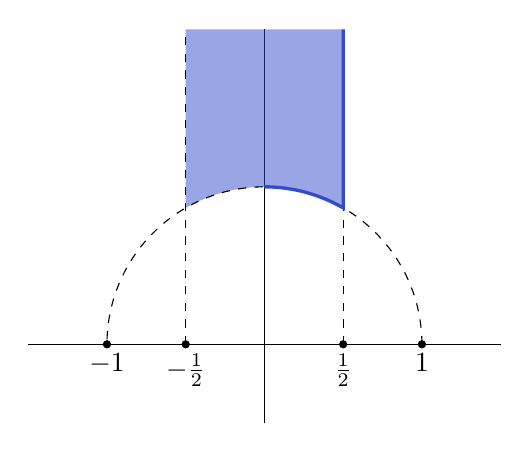
\begin{tikzpicture}
      \draw (-3, 0) -- (3, 0);

      \draw (0, -1) -- (0, 4);

      \node [circ] at (1, 0) {};
      \node [below] at (1, 0) {$\frac{1}{2}$};

      \node [circ] at (2, 0) {};
      \node [below] at (2, 0) {$1$};

      \node [circ] at (-1, 0) {};
      \node [below] at (-1, 0) {$-\frac{1}{2}$};

      \node [circ] at (-2, 0) {};
      \node [below] at (-2, 0) {$-1$};

      \fill [opacity=0.5, mblue] (1, 4) -- (1, 1.732) arc (60:120:2) -- (-1, 4);

      \draw [dashed] (2, 0) arc (0:180:2);

      \draw [dashed] (1, 0) -- (1, 4);
      \draw [dashed] (-1, 0) -- (-1, 4);
      \draw [very thick, mblue] (1, 4) -- (1, 1.732) arc (60:90:2);
    \end{tikzpicture}
  \end{center}
  Then $\mathcal{D}$ is a \term{fundamental domain} for the action of $\bar{\Gamma}$ on $\H$, ie. every orbit contains exactly one element of $\mathcal{D}$.

  The stabilizer of $z \in \mathcal{D}$ in $\Gamma$ is \emph{trivial} if $z \not\in \{i, \rho = e^{\pi i/3}\}$, and
  \[
    \bar{\Gamma}_i = \bra S\ket \cong \frac{\Z}{2Z},\quad \Gamma_\rho = \bra TS\ket \cong \frac{\Z}{3\Z}.
  \]
  Finally, $\bar \Gamma = \bra S, T \ket = \bra S, TS\ket$.
\end{thm}
In fact, $\bar\Gamma$ is generated \emph{freely} by $S, TS$, except for the relation $S^2 = 2, (TS)^3 = 1$.

\begin{proof}
  Let $\bar{\Gamma}^* = \bra S, T\ket \subseteq \bar{\Gamma}$. We will show that if $z \in \H$, then there exists $\gamma \in \bar\Gamma^*$ such that $\gamma(z) \in \mathcal{D}$.

  Since $z \not \in \R$, we know $\Z + \Z z = \{cz + d: c, d \in \Z\}$ is a discrete subgroup of $\C$. So we know
  \[
    \{|cz + d|: c, d \in \Z\}
  \]
  is a discrete subset of $\R$. So
  \[
    \left\{\Im \gamma(z) = \frac{\Im (z)}{|cz + d|^2}: \gamma =
    \begin{pmatrix}
      a & b\\
      c & d
    \end{pmatrix} \in \bar\Gamma^*\right\}
  \]
  is a discrete subset of $\R_{>0}$, bounded above. So there is some $\gamma \in \bar{\Gamma}^*$ with $\Im \gamma(z)$ \emph{maximal}.

  Replacing $\Gamma$ by $T^n \gamma$ for sutiable $n$, we may assume $|\Re \gamma(z)| \leq \frac{1}{2}$.

  If $|\gamma(z)| < 1$, then
  \[
    \Im S \gamma(z) = \Im \frac{-1}{\gamma(z)} = \frac{\Im \gamma(z)}{|\gamma(z)|^2} > \Im \gamma(z),
  \]
  which is impossible. So we know $|\gamma(z)| \geq 1$. So we know $\gamma(z)$ lives in the closure of $\mathcal{D}$.

  Now if $\Re(\gamma(z)) = -\frac{1}{2}$, then $T \gamma(z)$ has real part $+\frac{1}{2}$, and so $T(\gamma(z)) \in \mathcal{D}$.

  Now if $-\frac{1}{2} < \Re(z) < 0$ and $|\gamma(z)| = 1$, then $|S\gamma(z)| = 1$ and $0 < \Re S\gamma(z) < \frac{1}{2}$, ie. $S \gamma(z) \in \mathcal{D}$.

  \separator

  We shall next show that if $z, z' \in \mathcal{D}$,and $z' = \gamma(z)$ for $\gamma \in \bar{\Gamma}$, then $z = z'$ and either $\gamma = 1$ or $z = i, \gamma = S$ or $z = \rho, \gamma = TS$ or $(TS)^2$. It is clear that this proves everything.

  To show this, we wlog
  \[
    \Im (z') = \frac{\Im z}{|cz + d|^2} \geq \Im z
  \]
  where
  \[
    \gamma =
    \begin{pmatrix}
      a & b\\
      c & d
    \end{pmatrix},
  \]
  and we also wlog $c \geq 0$.

  Therefore we know that $|cz + d| \leq 1$. In particular, we know
  \[
    1 \geq \Im(cz + d) = c \Im (z) \geq c \frac{\sqrt{3}}{2}
  \]
  since $z \in \mathcal{D}$. So $c = 0$ or $1$.

  \begin{itemize}
    \item If $c = 0$, then
      \[
        \gamma = \pm
        \begin{pmatrix}
          1 & m\\
          0 & 1
        \end{pmatrix}
      \]
      for some $m \in \Z$, and this $z' = z + m$. But this is clearly impossible. So we must have $m = 0$, $z = z'$, $\gamma = 1 \in \PSL_2(\Z)$.

    \item If $c = 1$, then we know $|z + d| \leq 1$. So $z$ is at distance $1$ from an integer. As $z \in \mathcal{D}$, the only possibilities are $d = 0$ or $-1$.

      \begin{itemize}
        \item If $d = 0$, then we know $|z| = 1$. So
          \[
            \gamma =
            \begin{pmatrix}
              a & -1\\
              1 & 0
            \end{pmatrix}
          \]
          for some $a \in \Z$. Then $z' = a - \frac{1}{z}$. Then
          \begin{itemize}
            \item either $a = 0$, which forces $z = i$, $\gamma = S$; or
            \item $a = 1$, and $z' = 1 - \frac{1}{z}$, which implies $z = z' = \rho$ and $\gamma = TS$.
          \end{itemize}
        \item If $d = -1$, then by looking at the picture, we see that $z = \rho$. Then
          \[
            |cz + d| = |z - 1| = 1,
          \]
          and so
          \[
            \Im z' = \Im z = \frac{\sqrt{3}}{2}.
          \]
          So we have $z' = \rho$ as well. So
          \[
            \frac{a \rho + b}{\rho - 1} = \rho,
          \]
          which implies
          \[
            \rho^2 - (a + 1) \rho - b = 0
          \]
          So $\rho = -1, a = 0$, and $\gamma = (TS)^2$.
      \end{itemize}
  \end{itemize}
\end{proof}

Note that $S$ and $T$ identify the portions of the boundary of $\mathcal{D}$. So the quotient $\bar{\Gamma}\setminus \H$ is obtained by identifying the boundary points of $\mathcal{D}$ using $T$ and $S$, and we get something homeomorphic to a disk.

Note that this proof is the same as the proof of reduction theory for binary positive definite binary quadratic forms.

An important consequence of this is that the quotient $\Gamma \setminus \H$ has \emph{finite invariant measure}.
\begin{prop}
  The measure
  \[
    \d \mu = \frac{\d x\;\d y}{y^2}
  \]
  is invariant under $\PSL_2(\R)$. If $\Gamma \subseteq \PSL_2(\Z)$ is of finite index, then $\mu(\Gamma\setminus \H) < \infty$.
\end{prop}

\begin{proof}
  Consider the $2$-form associated to $\mu$, given by
  \[
    \eta = \frac{\d x \wedge \d y}{y^2} = \frac{i \d z \wedge \d \bar{z}}{2 (\Im z)^2}.
  \]
  We now let
  \[
    \gamma =
    \begin{pmatrix}
      a & b\\
      c & d
    \end{pmatrix} \in \SL_2(\R).
  \]
  Then we have
  \[
    \Im \gamma(z) = \frac{\Im z}{|cz + d|^2}.
  \]
  Moreover, we have
  \[
    \frac{\d \gamma(z)}{\d z} = \frac{a(cz + d) - c(az + b)}{(cz + d)^2} = \frac{1}{(cz + d)^2}.
  \]
  So $\eta$ is invariant under $\gamma$.

  Now if $\bar\Gamma \leq \PSL_2(\Z)$ has finite index, then we can write
  \[
    \PSL_2(\Z) = \coprod_{i = 1}^n \bar\gamma \gamma_i,
  \]
  where $n = (\PSL_2(\Z) \bar\Gamma)$, then a fundamental domain for $\bar\Gamma$ is just
  \[
    \bigcup_{i = 1}^n  \gamma_i(\mathcal{D}),
  \]
  and so
  \[
    \mu(\bar\Gamma \setminus H) = \sum \mu(\gamma_i \mathcal{D}) = n \mu(\mathcal{D}),
  \]
  and we can directly compute
  \[
    \mu(\mathcal{D}) = \int_\mathcal{D} \frac{\d x\; \d y}{y^2} \leq \int_{x = -\frac{1}{2}}^{x = \frac{1}{2}}\int_{y = \sqrt{2}/2}^{y = \infty} \frac{\d x\;\d y}{y^2} < \infty.
  \]
\end{proof}
It is an easy exercise to show that we actually have
\[
  \mu(\mathcal{D}) = \frac{\pi}{3}.
\]
\subsubsection*{Some subgroups of \texorpdfstring{$\SL_2(\Z)$}{SL2(Z)}}

\begin{defi}[Principal congruence subgroup]\index{$\Gamma(N)$}
  For $N \geq 1$, the \term{principal congruence subgroup} of level $N$ is
  \[
    \Gamma(N) = \{\gamma \in \SL_2(\Z) : \gamma \equiv I \pmod N\} = \ker (\SL_2(\Z) \to \SL_2(\Z/N\Z)).
  \]
  Any $\Gamma \subseteq \SL_2(\Z)$ containing some $\Gamma(N)$ is called a \emph{congruence subgroup}, and its \term{level} is the smallest $N$ such that $\Gamma \supseteq \Gamma(N)$
\end{defi}
This is a normal subgroup of finite index.
\begin{eg}
  We have
  \[
    \Gamma_0(N) =\left\{
      \begin{pmatrix}
        a & b\\
        c & d
      \end{pmatrix}
    \in \SL_2(\Z): c \equiv 0\pmod N\right\}
  \]
  and 
  \[
    \Gamma_1(N) =\left\{
      \begin{pmatrix}
        a & b\\
        c & d
      \end{pmatrix}
    \in \SL_2(\Z): c \equiv 0, d\equiv 1 \pmod N\right\}.
  \]
  We similarly define $\Gamma^0(N)$ and $\Gamma^1(N)$ to be the transpose of $\Gamma_0(N)$ and $\Gamma_1(N)$ respectively.
\end{eg}
Note that ``almost all'' subgroups of $\SL_2(\Z)$ are \emph{not} congruence subgroups (however, $2$ is just a special case. For $n> 2$, they are all are congruence).

We can now define a modular form.
\section{Modular forms of level 1}
Note that we have $\SL_2(\Z) = \Gamma(1)$.
\begin{defi}[Modular form of level 1]\index{modular form}\index{modular form!level 1}
  A holomorphic function $f: \H \to \C$ is a \emph{modular form of weight $k \in \Z$ and level $1$} if
  \begin{enumerate}
    \item For any
      \[
        \gamma =
        \begin{pmatrix}
          a & b\\
          c & d
        \end{pmatrix} \in \Gamma(1),
      \]
      we have
      \[
        f(\gamma)z = (cz + d)^k f(z).
      \]
    \item $f$ is holomorphic at $\infty$ (to be defined precisely later)
  \end{enumerate}
\end{defi}

Note that if we take $\gamma = -I$, then we get
\[
  f(z) = (-1)^k f(z).
\]
So if $k$ is odd, then $f \equiv 0$. So they only exist for even weights.

Also, since we know $\bar\Gamma = \bra S, T\ket$, and also we will see below that
\[
  f(z) \mapsto (cz + d)^{-k} f(\gamma(z))
\]
is a \emph{group action} of $\Gamma(1)$ on functions on $\H$. So the condition (i) is equivalent to
\[
  f(z + 1) = f(z),\quad f(-1/z) = z^k f(z).
\]
What do we mean by (ii)? We write $q = e^{2\pi i z}$\index{$q$} (which is a notation we will use throughout), so $z \in \H$ iff $0 < |q| < 1$. Then by (i), since we know $f(z + 1) = f(z)$, it follows that $f(z)$ only depends on $q$. So there exists a holomorphic function $\tilde{f}(q)$ on $\{0< |q| < 1\}$ such that
\[
  \tilde{f}(e^{2\pi i z}) = f(z).
\]
Explicitly, we can write
\[
  \tilde{f}(q) = f\left(\frac{1}{2\pi i} \log q\right).
\]
Now $\tilde{f}$ is a holomorphic function on a punctured disk. So we have a Laurent expansion
\[
  \tilde{f}(q) = \sum_{n = -\infty}^\infty a_n (f) q^n,
\]
called the \term{Fourier expansion} or \term{$q$-expansion} of $f$. We say $f$ is meromorphic (resp. holomorphic) at $\infty$ if $\tilde{f}$ is meromorphic (resp. holomorphic) at $q = 0$.

In other words, it is meromorphic at $\infty$ if $a_n(f) = 0$ for $n$ sufficiently negative, and holomorphic if $a_n(f) = 0$ for all $n \geq 0$. The latter just says $f(z)$ is bounded as $\Im(z) \to \infty$.

Some more terminology:
\begin{defi}[Cusp form]\index{cusp form}\index{modular form!cusp form}
  A modular form $f$ is a \emph{cups form} if the constant term $a_0(f)$ is $0$.
\end{defi}

In other words, we have
\[
  \tilde{f} = \sum_{n\geq 1} a_n(f) q^n.
\]
From now on, we will drop the $\tilde{\;}$, which should not cause confusion.

\begin{defi}[Weak modular form]\index{weak modular form}\index{modular form!weak}
  A \emph{weak modular form} is a holomorphic form on $\H$ satisfying (i) which is \emph{meromorphic} at $\infty$.
\end{defi}
We will use these occasionally.

Why do we care about modular forms? And also, are there actually modular forms? It turns out there are many, and they happen to be very interesting.

The first example we have is the Eisenstein. This has its origin in the theory of elliptic functions, but we will not go into that.

\begin{defi}[Eisenstein series]\index{Eisenstein series}
  Let $k \geq 4$ be even. We define
  \[
    G_k(z) = \sum_{m, n \in \Z, (m, n) \not= (0, 0)} \frac{1}{(mz + n)^k} = \sum_{(m, n) \in \Z^2}' \frac{1}{(mz + n)^k}.
  \]
\end{defi}
Here the $\sum'$ denotes that we are omitting $0$.

\begin{thm}
  $G_k$ is a modular form of weight $k$ and level $1$. Moreover, its $q$-expansion is
  \[
    G_k(z) = 2 \zeta(k) \left(1 - \frac{2k}{B_k} \sum_{n \geq 1}  \sigma_{k - 1}(n) q^n\right),\tag{$1$}
  \]
  where
  \[
    \sigma_r(n) = \sum_{1 \leq d \mid n} d^r.
  \]
\end{thm}

The first thing to prove is that the series actually converges absolutely for $k \geq 4$ (actually for $k \geq 3$, but the series is identically zero if $k$ is odd).

As $z \not \in \R$, we know $\{1, z\}$ is an $\R$-basis for $\C$. We will prove the following more general result.
\begin{prop}
  Let $(e_1, \cdots, e_d)$ be some basis for $\R^d$. Then if $r \in \R$, the series
  \[
    \sum'_{\mathbf{m} \in \Z^d} \|m_1 e_1 + \cdots + m_d e_d\|^{-r}
  \]
  converges iff $r > d$.
\end{prop}

\begin{proof}
  The function
  \[
    (x_i) \in \R^d \mapsto \left\|\sum_{i = 1} x_i e_i \right\|
  \]
  is a norm on $\R^d$. As any $2$ norms on $\R^d$ are equivalent,  we know this is equal to the sup norm $\|\ph\|_\infty$. So the series converges iff the corresponding series
  \[
    \sum_{\mathbf{m} \in \Z^d}' \|\mathbf{m}\|_\infty^{-r}
  \]
  converges. But if $1 \leq N \leq Z$, then the number of $\mathbf{m} \in \Z^d$ such that $\|\mathbf{m}\|_\infty = N$ is $(2N + 1)^d - (2N - 1)^d \sim 2^d d N^{d - 1}$. So the series converges iff
  \[
    \sum_{N \geq 1} N^{-r} N^{d - 1}
  \]
  converges, which is true iff $r > d$.
\end{proof}

\begin{proof}[Proof of theorem]
  Then convergence of the Eisenstein series by applying this to $\R^2 \cong \C$. So the series is absolutely convergent. Therefore we can simply compute
  \[
    G_k(z + 1) = \sum_{m, n}' \frac{1}{(mz + (m + n))^k} = G_k(z).
  \]
  Also we can compute
  \[
    G_k\left(-\frac{1}{z}\right) = \sum_{m, n}' = \frac{z^k}{(-m + nz)^k} = z^k G_k(z).
  \]
  So $G_k$ satisfies the invariance property. To show that $G_k$ is holomorphic, and holomorphic at infinity, we'll derive the $q$-expansion $(1)$.
\end{proof}

\begin{lemma}
  \[
    \sum_{n = \infty}^\infty \frac{1}{(n + w)^k} = \frac{(-2\pi i)^k}{(k - 1)!} \sum_{d = 1}^\infty d^{k - 1} e^{2\pi i d w}
  \]
  for any $w \in \H$ and $k \geq 2$.
\end{lemma}
There are (at least) two ways to prove this. One of this is to use the series for the cotangent, but here we will use Poisson summation.

\begin{proof}
  Let
  \[
    f(x) = \frac{1}{(x + w)^k}.
  \]
  We compute
  \[
    \hat{f}(y) = \int_{-\infty}^\infty \frac{e^{-2\pi i x y}}{(x + w)^k}\;\d x.
  \]
  We replace this with a contour integral. We see that this has a pole at $-w$. If $y > 0$, then we close the contour downwards, and we have
  \[
    \hat{f}(y) = -2\pi i \Res_{z = -w} \frac{e^{-2\pi i y z}}{(z + w)^k} = -2\pi i \frac{(-2\pi i y)^{k - 1}}{(k - 1)!} e^{2\pi i yw}.
  \]
  If $y \leq 0$, then we close in the upper half plane, and since there is no pole, we have $\hat{f}(y) = 0$. So we have
  \[
    \sum_{n = -\infty}^\infty \frac{1}{(n + w)^k} = \sum_{n \in \Z} f(n) = \sum_{d \in \Z} \hat{f}(d) = \frac{(-2\pi i)^k}{(k - 1)!} \sum_{d \geq 1} d^{k - 1} e^{2\pi i d w}
  \]
  by Poisson summation formula.
\end{proof}

Note that when we proved the Poisson summation formula, we required $f$ to decrease very rapidly at infinity, and our $f$ does not satisfy that condition. However, we can go back and check that the proof still works in this case.

Now we get back to the Eisentein series. We have
\begin{align*}
  G_k(z) &= 2 \sum_{n \geq 1} \frac{1}{n^k} + 2 \sum_{m \geq 1} \sum_{n \in \Z} \frac{1}{n + mz)^k}\\
  &= 2 \zeta(k) + 2 \sum_{m \geq 1} \frac{(2\pi i )6k}{(k - 1)!} \sum_{d \geq 1} q^{dm}.\\
  &= 2 \zeta(k) + 2 \frac{(2\pi i)^k}{(k - 1)!} \sum_{n \geq 1} \sigma_{k - 1}(n) q^n.
\end{align*}
Then the result follows from the fact that
\[
  \zeta(k) = -\frac{1}{2} (2\pi i)^k \frac{B_k}{k!}.
\]
So we see that $G_k$ is holomorphic in $\H$, and is also holomorphic at $\infty$.

It is convenient to introduce a \emph{normalized} Eisenstein series
\begin{defi}[Normalized Eisenstein series]\index{normalized Eisenstein series}\index{Eisenstein series!normalized}
  We define
  \begin{align*}
    E_k(z) &= (2 \zeta(k))^{-1} G_k(z) \\
    &= 1 - \frac{2k}{B_k} \sum_{n \geq 1} \sigma_{k - 1}(n) q^n\\
    &= \frac{1}{2} \sum_{\substack{(m, n) = 1}{m, n \in \Z}} \frac{1}{(mz + n)^k}.
  \end{align*}
\end{defi}
The last line follows by taking out any common factor of $m, n$ in the series defining $G_k$.

\begin{eg}
  \[
    B_2 = \frac{1}{6},\quad B_4 = \frac{-1}{30},\quad B_6 = \frac{1}{42},\quad B_8 = \frac{-1}{30},\quad B_{10} = \frac{5}{66}, \quad B_{12} = \frac{-631}{2730},\quad B_{14} = \frac{7}{6}.
  \]
  Using these, we find
  \begin{align*}
    E_4 &= 1 + 240 \sum \sigma_3(n) q^n\\
    E_6 &= 1 - 504 \sum \sigma_5 (n) q^n\\
    E_8 &= 1 + 480 \sum \sigma_7(n) q^n\\
    E_{10} &= 1 - 264 \sum \sigma_9(n) q^n\\
    E_{12} &= 1 + \frac{65520}{691} \sum \sigma_{11}(n) q^n\\
    E_{14} = 1 - 24 \sum \sigma_{13}(n) q^n.
  \end{align*}
\end{eg}
We notice that there is a simple pattern for $k \leq 14$, except for $k = 12$.

There is another interpretation of Eisenstein series, which is more group theoretic, but before that, we introduce some useful terminology.

\begin{defi}[Slash operator]\index{slash operator}
  Let
  \[
    \begin{pmatrix}
      a & b\\
      c & d
    \end{pmatrix} = \gamma \in \GL_2(\R)^+,\quad z \in \H,
  \]
  and $f: \H \to \C$ any function. We also write
  \[
    j(\gamma, z) = cz + d.
  \]
  We define the \emph{slash operator} to be
  \[
    (f\underset{k}{|} \gamma) (z) = (\det \gamma)^{k/2} j(\gamma, z)^{-k} f(\gamma(z)).
  \]
\end{defi}
Note that some people leave out the $\det \gamma^{k/2}$ factor, but if we have it, then whenever $\gamma = Ia$, then
\[
  f\underset{k}{|} \gamma = \sgn(a)^k f.
\]
In this notation, then condition (i) for $f$ to be a modular form is just
\[
  f\underset{k}{|}\gamma = f
\]
for all $\gamma \in \SL_2(\Z)$.

Now note that
\[
  \gamma
  \begin{pmatrix}
    z\\1
  \end{pmatrix}
  = j(\gamma, z)
  \begin{pmatrix}
    \gamma(z)\\1
  \end{pmatrix}.\tag{$*$}
\]
\begin{prop}\leavevmode
  \begin{enumerate}
    \item $j(\gamma\delta, z) = j(\gamma, \delta(z)) j(\delta, z)$ (thus $j$ is a $1$-cocycle)
    \item $j(\gamma^{-1}, z) = j (\gamma, \gamma^{-1}(z))^{-1}$
    \item $\gamma: \varphi \mapsto f\underset{k}{|} \gamma$ is a (right) action of $G = \GL_2(\R)^+$ on functions on $\H$. In other words, 
      \[
        f\underset{k}{|} \gamma \underset{k}{|} \delta = f\underset{k}{|}(\gamma\delta).
      \]
  \end{enumerate}
\end{prop}
Note that this implies that if if $\Gamma \leq \GL_2(\R)^+$ and $\Gamma = \bra \gamma_1, \cdots, \gamma_m\ket$ then
\[
  f\underset{k}{|} \gamma = f\Longleftrightarrow f\underset{k}{|} \gamma_i = f\text{ for all }i = 1, \cdots, m.
\]
\begin{proof}\leavevmode
  \begin{enumerate}
    \item We have
      \[
        j(\gamma\delta, z)
        \begin{pmatrix}
          \gamma\delta(z)\\
          1
        \end{pmatrix} =
        \gamma\delta
        \begin{pmatrix}
          z\\1
        \end{pmatrix}
        =
        j(\delta, z) \gamma
        \begin{pmatrix}
          \delta(z)\\
          1
        \end{pmatrix}
        =
        j(\delta, z) j(\gamma, \delta(z))
        \begin{pmatrix}
          z\\1
        \end{pmatrix}
      \]
    \item Take $\delta = \gamma^{-1}$.
    \item We have
      \begin{align*}
        ((f\underset{k}{|} \gamma) \underset{k}{|} \delta) &= (\det \delta)^{k/2} j(\delta, z)^{-k} (f\underset{k}{|} \gamma) (\delta(z))\\
        &= (\det \delta)^{k/2} j(\delta, z)^{-k} (\det \gamma)^{k/2} j(\gamma, \delta(z))^{-k} f(\gamma\delta(z))\\
        &= (\det \gamma \delta)^{k/2} j(\gamma \delta, z)^{-k} f(\gamma\delta(z))\\
        &= (f\underset{k}{|} \gamma\delta) (z).
      \end{align*}
  \end{enumerate}
\end{proof}
Back the the Eisenstein series. $G_k$ arise naturally in elliptic functions, which are ceofficients in the series expansion of Weierstrass $\wp$ function. % fix

Another group-theoretic interpretation, which generalizes in many ways. Consider
\[
  \Gamma(1)_\infty = \left\{
    \pm
    \begin{pmatrix}
      1 & n\\
      0 & 1
    \end{pmatrix}: n \in \Z
  \right\} \leq \Gamma(1) = \SL_2(\Z),
\]
which is the stabilizer of $\infty$. If
\[
  \delta = \pm
  \begin{pmatrix}
    1 & n\\
    0 & 1
  \end{pmatrix}
  \in \Gamma(1)_\infty,
\]
then we have
\[
  j(\delta\gamma, z) = j(\delta, \gamma(z)) j(\gamma, z) = \pm j(\gamma, z).
\]
So $j(\gamma, z)^2$ depends only on the coset $\Gamma(1)_\infty \gamma$. We can also check that if
\[
  \gamma =
  \begin{pmatrix}
    a & b\\
    c & d
  \end{pmatrix},\quad
  \gamma = 
  \begin{pmatrix}
    a' & b'\\
    c' & d'
  \end{pmatrix} \in \Gamma(1),
\]
then $\Gamma(1)_\infty \gamma = \Gamma(1)_\infty \gamma'$ iff $(c, d) = \pm (c', d')$.

Moreover, $\gcd(c, d) = 1 $ iff there  exists $a, b$ such that
\[
  \begin{vmatrix}
    a & b\\
    c & d
  \end{vmatrix} = 1.
\]
We therefore have 
\[
  E_k(z) = \sum_{\gamma \in \Gamma(1)_\infty \setminus \Gamma(1)} j(\gamma, z)^{-k},
\]
where we sum over (any) coset representatives of $\Gamma(1)_\infty$.

We can generalize this in two ways. We can either replace $j$ with some other appropriate function, or change the groups.
\printindex
\end{document}
